\documentclass{beamer}
\usetheme[numbering=fraction]{metropolis}           % Use metropolis theme

\newcommand{\supp}{\text{supp }}
\newcommand{\prox}{\text{Prox}}
\renewcommand{\div}{\text{div}}
\newcommand{\proj}{\text{Proj}}

\input{/home/tim/Documents/Ecole/modele_diapositives.tex}

\DeclareMathOperator*{\argmax}{arg\,max}
\DeclareMathOperator*{\argmin}{arg\,min}

\usepackage{multimedia}
\usepackage{subcaption}

\title{Transport Optimal\\Théorie et Applications}
\date{\today}
\author{Timothée Schmoderer}
\institute{INSA Rouen Normandie\\Département Génie Mathématique}

\begin{document}
  \maketitle
  \begin{frame}
	\vspace{1.cm}
  \tableofcontents
  \end{frame}

  
  \section{Introduction}
  \begin{frame}{Introduction}
  	\only<1-3>{
    \begin{enumerate}
    	\item<1-3> 1781 - Gaspard Monge : \emph{Mémoire sur la théorie des Déblais et des remblais}\\
    	\item<2-3> 1940 - Leonid Kantorovitch : Formulation moderne
    	\item<3>   1999 - J.D. Benamou et Y. Brenier : Nouveaux développements
    \end{enumerate}
    }
    \only<2>{
    \vspace{-1cm}
    \begin{figure}
    	\begin{subfigure}[c]{0.3\linewidth}
    		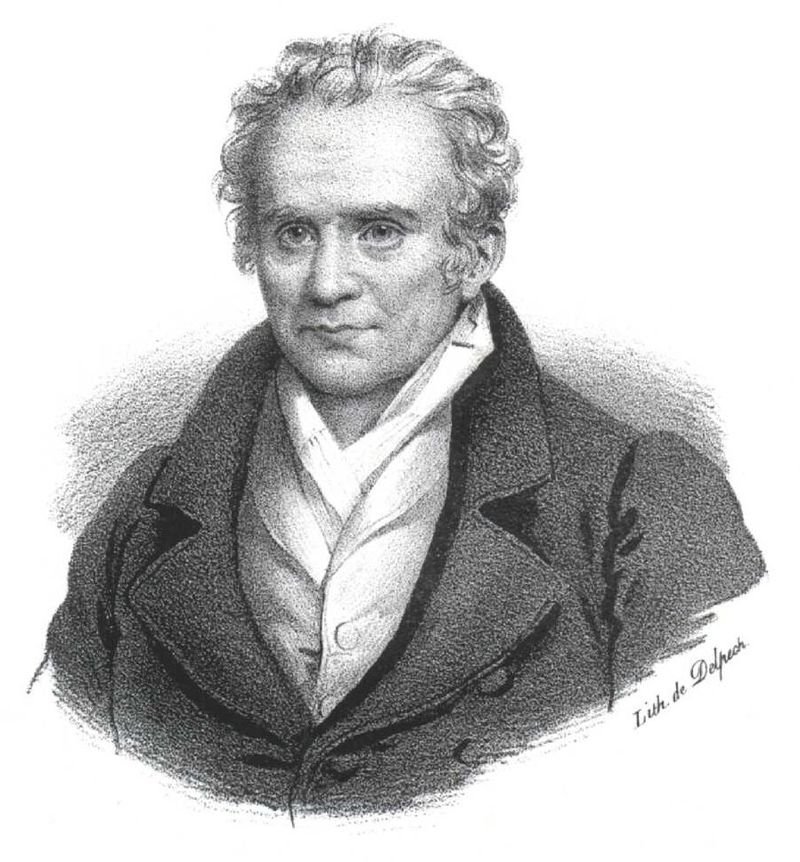
\includegraphics[width=\linewidth]{img/monge.jpg}
    		\caption{Gaspard Monge}
    	\end{subfigure}
    	~
    	\begin{subfigure}[c]{0.3\linewidth}
    		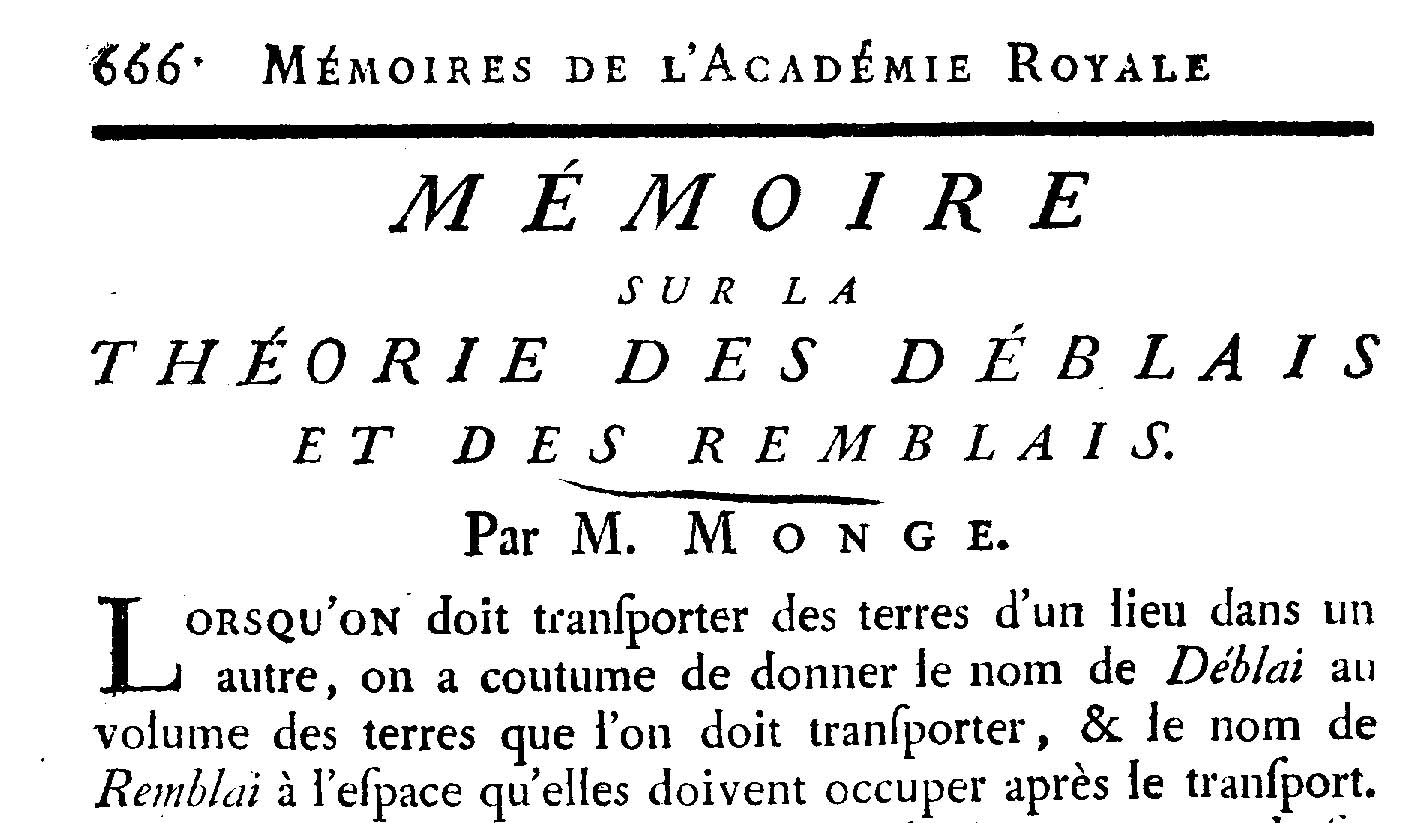
\includegraphics[width=\linewidth]{img/memoire.jpg}
    		\caption{Mémoire sur la théorie des déblais et remblais}
    	\end{subfigure}
    	~
    	\begin{subfigure}[c]{0.3\linewidth}
    		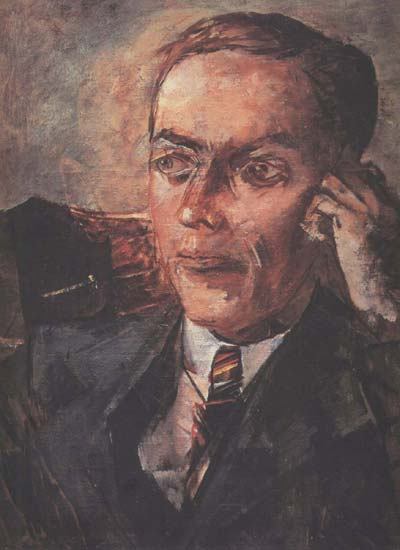
\includegraphics[width=\linewidth]{img/kantorovitch.jpg}
    		\caption{Leonid Kantorovitch}
    	\end{subfigure}
    \end{figure}
    }
    \only<3>{
    \begin{figure}
    	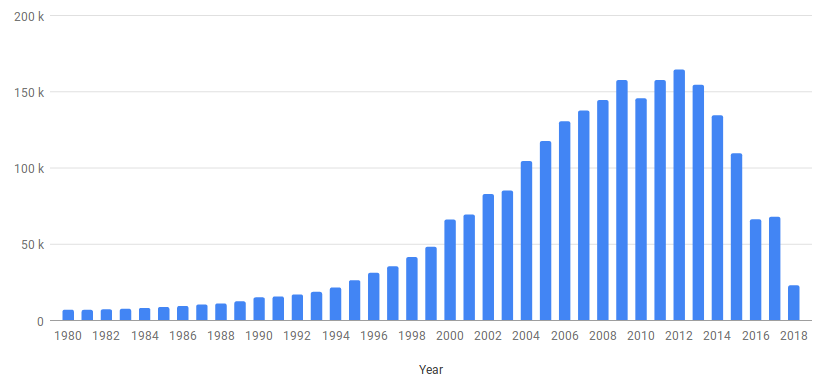
\includegraphics[width=0.8\linewidth]{img/trends.png}
    	\caption{Popularité des termes "Optimal Transport" ces 40 dernières années sur Google Scholar}
    \end{figure}
    }
    \only<4>{
    \begin{enumerate}
    	\item Benamou, Jean-David et Brenier, Yann, \emph{A computational fluid mechanics solution to the Monge-Kantorovich mass transfer problem}.
    	\item Papadakis, Nicolas et Peyr{\'e}, Gabriel et Oudet, Edouard, \emph{Optimal transport with proximal splitting}
    	\item Santambrogio, F., \emph{Optimal Transport for Applied Mathematicians: Calculus of Variations, PDEs, and Modeling}
    	\item Combettes PL., Pesquet JC, \emph{Proximal methods in signal processing}
    \end{enumerate}
    }
  \end{frame}
  
  \section{Théorie du Transport Optimal}
  \subsection{Définitions}
  \begin{frame}\frametitle{Le transport}
  \only<1>{
  	\begin{figure}
  		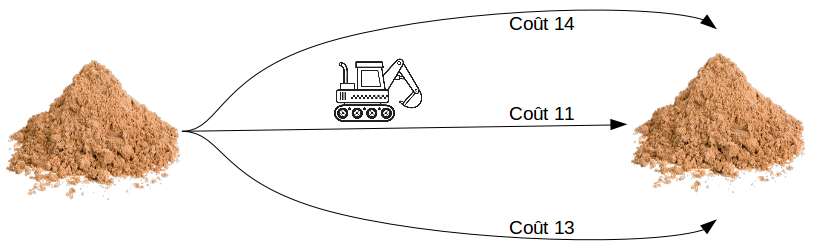
\includegraphics[width=\linewidth]{img/tractopelle.png}
  		\caption{\label{fig:tractopelle}Le transport optimal dans sa version vulgarisée}
	\end{figure}
	}
	\only<2>{
	\begin{definition}
		Soient deux mesures de probabilité $\mu$ sur $(\mathcal{X},\mathcal{B}(\mathcal{X}))$ et $\nu$ sur $(\mathcal{Y},	\mathcal{B}(\mathcal{Y}))$ munis de leur tribu borélienne. Un \textbf{transport} est une application $T\ :\ 		\mathcal{X}\rightarrow\mathcal{Y}$ qui envoie la mesure $\mu$ sur la mesure $\nu$. C'est à dire : 
		\begin{align}
			\forall B\in\mathcal{B}(\mathcal{Y}),\quad \mu(T^{-1}(B))=\nu(B)
			\label{eq:trspmesures}
		\end{align}
	Notons $T_{\#}\mu=\nu$
  	\end{definition}
  	}
  	\only<3>{
  	\begin{figure}[!h]
\centering
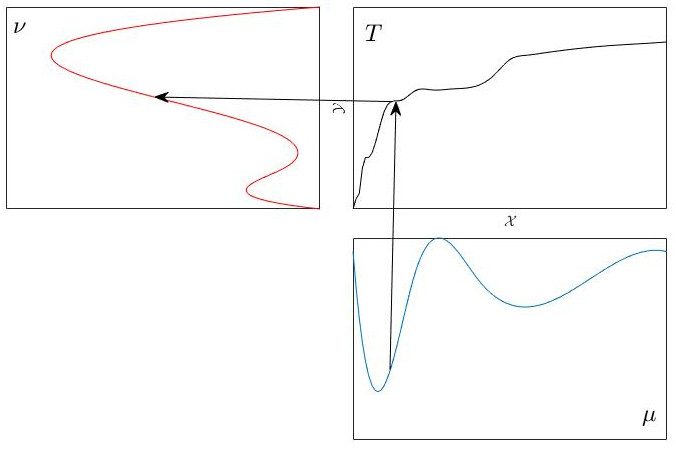
\includegraphics[width=0.7\linewidth]{img/transport.jpg}
\caption{\label{fig:illustrans}Illustration de l'application de transport}
\end{figure}
  	}
  \end{frame}
  
  \begin{frame}\frametitle{Le coût}
  \begin{definition}
Le coût est une application 
$$
\fonction{C}{\mathcal{X}\times\mathcal{Y}}{[0,+\infty]}{(x,y)}{C(x,y)}
$$
\end{definition}
  \end{frame}
  
  \begin{frame}\frametitle{Le problème de transport Optimal}
  \fbox{
  \parbox{\textwidth}{
  Étant données deux mesures de probabilités $\mu$ sur $\mathcal{X}$, $\nu$ sur $\mathcal{Y}$ et une application coût $C$, trouver une application de transport $T$ réalisant le 
	\begin{equation}
	\tag{MP}
	\inf\left\{M(T) := \int_{\mathcal{X}} C(x,T(x))\ d\mu (x), \quad T_{\#}\mu = \nu\right\}
	\label{eq:MP}
	\end{equation}
  }
}
  \end{frame}
  
  
  \subsection{Existence du transport Optimal}
  \begin{frame}\frametitle{Relaxation, Plan de transport optimal}
  \only<1>{
  	\fbox{
  \parbox{\textwidth}{
  Étant données deux mesures de probabilités $\mu$ et $\nu$ et un coût $C$, trouver la mesure $\pi$ réalisant le 
	\begin{equation}
	\tag{KP}
	\inf\left\{ K(\pi ) := \int_{\mathcal{X}\times\mathcal{Y}} C(x,y)\ d\pi (x,y), \quad \pi \in\Pi(\mu,\nu )\right\}
	\label{eq:KP}
	\end{equation}
	Où, $\Pi(\mu,\nu)$ est l'ensemble des plans de transports : 
	\begin{empheq}[left={ \Pi(\mu,\nu) = \empheqlbrace}]{align}
	  &  \pi \text{ une probabilité sur }\mathcal{X}\times\mathcal{Y}\nonumber \\
      &  \forall A\in\mathcal{B}(\mathcal{X}),\quad \pi (A\times\mathcal{Y}) = \mu(A) \label{eq:contrKP}\\
      &  \forall B\in\mathcal{B}(\mathcal{Y}),\quad \pi (\mathcal{X}\times B) = \nu(B)  \nonumber,
	\end{empheq}
  }
}
}
	\only<2>{
	\begin{figure}[!h]
\centering
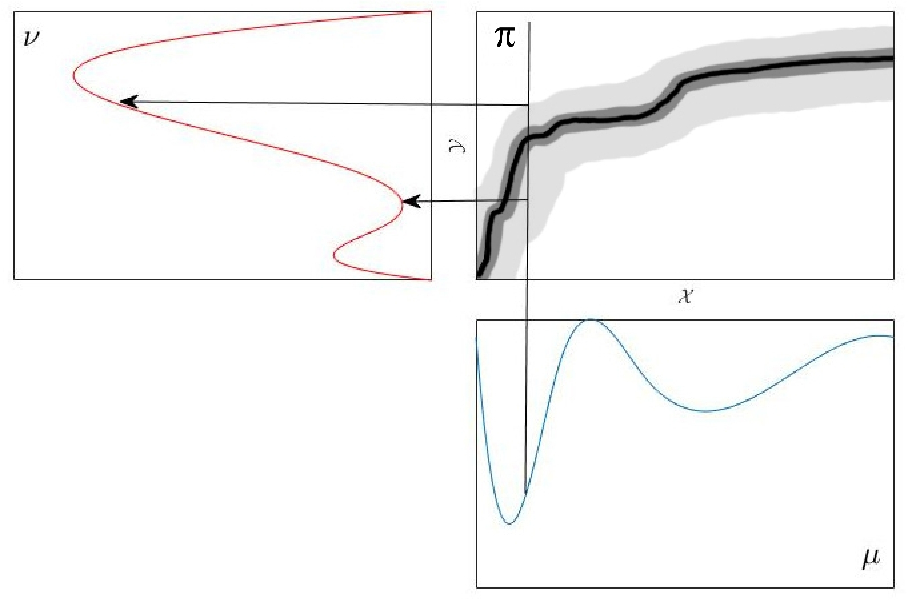
\includegraphics[width=0.6\linewidth]{img/transport_plan2.jpg}
\caption{Illustration de la notion de plan de transport\label{fig:plantransp}}
\end{figure}	
	}
  \end{frame}
  
  \begin{frame}\frametitle{Existence du plan de transport Optimal}
  	\begin{theoreme}{}
Soit $\mathcal{X}$ et $\mathcal{Y}$ des espaces métriques compacts. Supposons que le coût $C\ :\ \mathcal{X}\times\mathcal{Y}\rightarrow [0,+\infty]$ soit continue. Alors le problème \eqref{eq:KP} admet une solution.
\end{theoreme}
  \end{frame}
  
  
  \subsection{Formulation Duale}
  
  \begin{frame}\frametitle{Problème dual}
\only<1>{
  \fbox{
  \parbox{\textwidth}{
  Étant données deux mesures de probabilités $\mu$ et $\nu$ et un coût $C$, trouver deux fonctions continues, bornées $\phi$ et $\psi$ réalisant le 
	\begin{equation}
	\tag{DKP}
	\sup\left\{\int_{\mathcal{X}} \phi\ d\mu + \int_{\mathcal{Y}}\psi\ d\nu, \quad  (\phi,\psi)\in C_b(\mathcal{X})\times C_b(\mathcal{Y}),\quad \phi\oplus\psi \leq C \right\}
	\label{eq:DKP}
	\end{equation}
  }
}
}
\only<2>{
\begin{theoreme}{}
\label{thm:existDKP}
Supposons que $\mathcal{X}$ et $\mathcal{Y}$ soient compact et que $C$ est continue. Alors il existe une solution $(\phi,\psi)$ au problème \eqref{eq:DKP}.
\end{theoreme}
}
\only<3>{
\begin{theoreme}{}
\label{thm:dualite}
Les problèmes \eqref{eq:KP} et \eqref{eq:DKP} sont bien duaux l'un de l'autre :
\begin{align}
\min\eqref{eq:KP} = \max\eqref{eq:DKP}
\end{align}
\end{theoreme}
}
  \end{frame}
  
  
  \begin{frame}\frametitle{}
  \begin{theoreme}{Existence du transport optimal}
\label{thm:existtrasp}
Soient $\mu$ et $\nu$ des mesures de probabilités sur une domaine compact $\Omega$ de $\RR^n$ et un coût $C(x,y) = h(x-y)$, avec $h$ strictement convexe.\\ 
Alors il existe une solution $\pi$ au problème \eqref{eq:KP}. \\
De plus, $\pi$ est unique, de la forme $(Id,T)_{\#}\mu$ si $\mu$ est absolument continue et $\partial\Omega$ est $\mu$ - négligeable.\\
Enfin, une solution de \eqref{eq:DKP}, $\phi$ qui est liée à $T$ par :
\begin{align}
T(x) = x- (\partial h)^{-1}(\nabla\phi(x))
\end{align}
\end{theoreme}
  \end{frame}
  
  \subsection{Cas quadratique dans $\RR^n$}
  
  \begin{frame}\frametitle{Coût quadratique}
  	Prenons $C(x,y)=\frac{1}{2}\|x-y\|^2$. \\
  	\begin{theoreme}{}
Soient $\mu$ et $\nu$ des probabilités sur $\RR^n$ et $C(x,y)=\frac{1}{2}\|x-y\|^2$. Supposons que : 
\begin{enumerate}
\item $\int\|x\|^2d\mu$, $\int\|y\|^2d\nu<+\infty$
\item $\mu$ ne donne pas de masse aux hypersurfaces de classe $C^2$.
\end{enumerate}
alors il existe une unique application de transport optimal $T$, donnée par $T=\nabla u$ pour une fonction convexe $u$.
\end{theoreme}
  \end{frame}

  
  \begin{frame}\frametitle{Simplifications}
  Mettons nous dans $\RR^n$, prenons $\mu = f_0\ dx$ et $\nu = f_1\ dx$.
\only<1-2> { 
	\begin{align*}
	\forall B \in\mathcal{B}(\RR^n),\quad \int_B f_1(y)dy&=\int_{T^{-1}(B)} f_0(x) dx \\
	&= \int_B \sum_{x\in T^{-1}(y)} \left(\frac{f_0(x)}{|det\ \nabla T(x)|}\right)dy\\
	\Rightarrow\quad f_1(y) &= \sum_{x\in T^{-1}(y)} \left(\frac{f_0(x)}{|det\ \nabla T(x)|}\right)
	\end{align*}
}
\only<2>{ 
	\begin{equation}
	\tag{J}
	f_1(T(x)) = \frac{f_0(x)}{|det\ \nabla T(x)|}
	\label{eq:jacobienne}
	\end{equation}
}
\only<3>{
Dans le cas quadratique :
	\begin{equation}
	\tag{MA}
	f_1(\nabla u(x)) = \frac{f_0(x)}{det\ H u(x)}
	\label{eq:mongemapere}
	\end{equation}
}
\only<4>{
	Notons $\mathcal{T}(f_0,f_1)$ l'ensemble des applications qui vérifient \eqref{eq:jacobienne}.
	\begin{definition}{Métrique de Wasserstein}
	Pour les coûts de transport de la forme $C(x,y) = \|x - y\|^p$, nous pouvons définir une métrique entre $f_0$ et 	$f_1$ par
	\begin{align*}
	W(f_0,f_1)^p=\min_{T\in\mathcal{T}(f_0,f_1)} \int \|x-T(x)\|^pf_0(x)\ dx
	\end{align*} 
	\end{definition}
}
  \end{frame}

  
  
  \section{Formulation de Benamou et Brenier}
  \begin{frame}
  \begin{theoreme}{Benamou, Brenier}
	Soient $f_0$ et $f_1$ deux densités de probabilité assez régulières. Alors, 
	\begin{align*}
	\min_{T\in\mathcal{T}(f_0,f_1)} \int\|x-T(x)\|^2f_0dx =\min_{(f,v)\in\mathcal{C}_v}\int_{\RR^n}\int_0^1 f(t,x)\|v(t,x)\|^2dtdx
	\end{align*}
	Avec,
	\begin{align*}
	f(t,x)\ :&\ \RR\times\RR^n\rightarrow \RR \quad \text{la densité}\\
	v(t,x)\ :&\ \RR\times\RR^n\rightarrow \RR^n \quad \text{champ de vecteurs vitesses}
	\end{align*}
	et 
	\begin{align*}
	C_v=\left\{(f,v)\ |\ \frac{\partial f}{\partial t} + \text{div}_x (fv) =0,\ f(0,\cdot) = f_0,\ f(1,\cdot)=f_1 \right\}
	\end{align*}
	\end{theoreme}
  \end{frame}
  
	\section{Théorie des opérateurs proximaux}  
  \begin{frame}\frametitle{Sous différentiel}
  \only<1>{
\textbf{Notation :}Le domaine d'une fonction $f:\ \RR^n\longrightarrow\ ]-\infty,+\infty]$ est $\mathcal{D}(f) = \{ x\in\RR^n\ |\ f(x) < +\infty \} $.\\
Notons $\Gamma_0(\RR^n)$ l'ensemble des fonctions convexes semi-continues inférieurement à valeurs dans $]-\infty,+\infty]$ telles que $\mathcal{D}(f) \neq \emptyset$.
  }
  \only<2>{
  \begin{definition}
Soit $f\in\Gamma_0(\RR^n)$, le sous - différentiel de $f$ est l'application suivante,
$$
\fonction{\partial f}{\RR^n}{\mathcal{P}(\RR^n)}{x}{\left\{ u\in\RR^n\ |\ \forall y\in\RR^n,\ \langle u,y-x\rangle +f(x)\leq f(y) \right\}}
$$ 
Avec $\mathcal{P}(\RR^n)$, l'ensemble des parties de $\RR^n$.
\end{definition}
}
\only<3>{
\begin{figure}
\centering
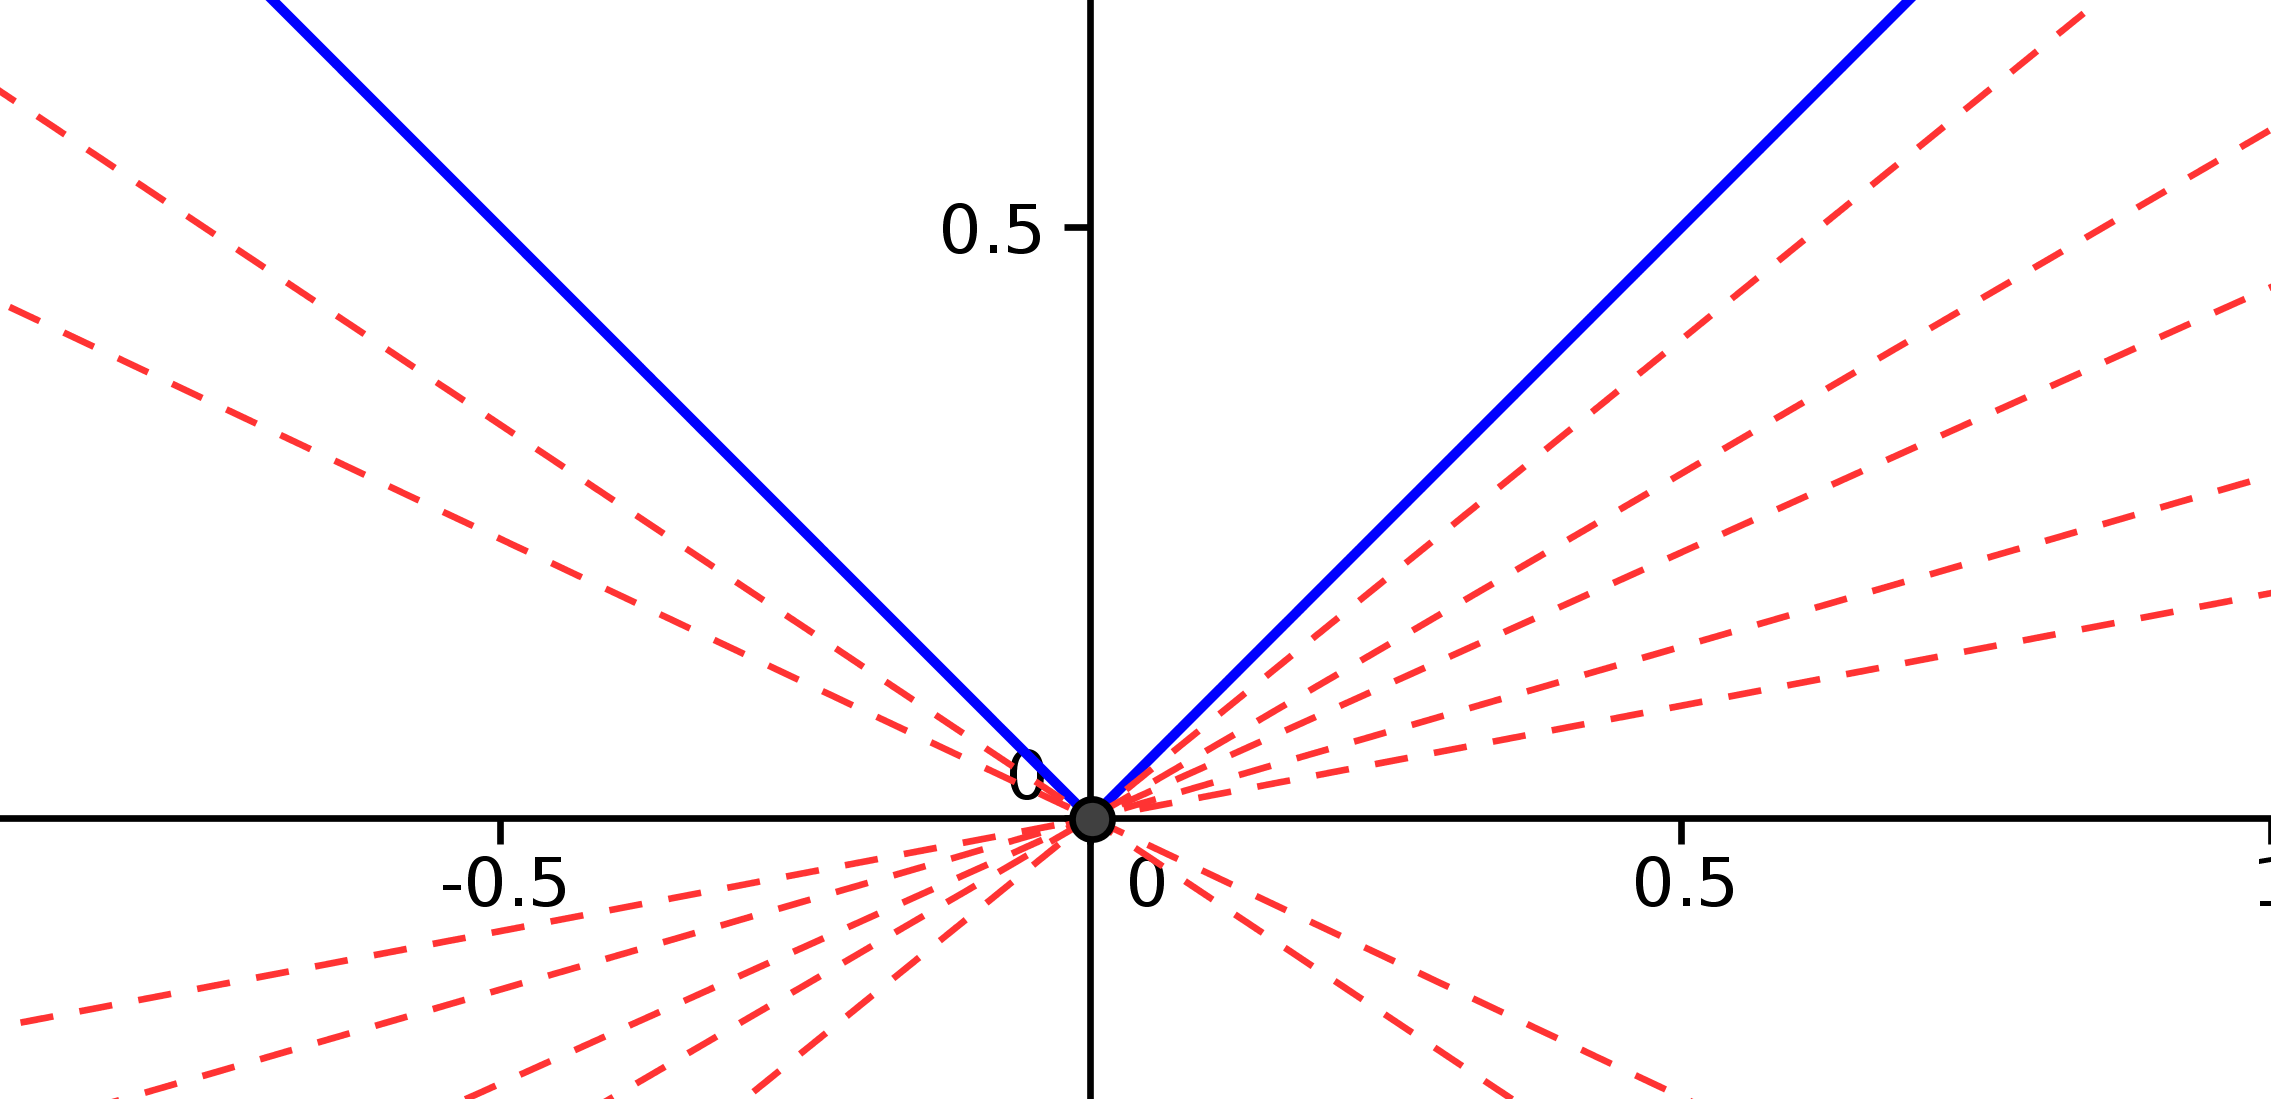
\includegraphics[width=0.9\linewidth]{img/sub_gradient.png}
\caption{\label{fig:subgradient}Illustration du sous - différentiel de $|x|$ en $0$}
\end{figure}
}
\only<4>{
\begin{propriete}
Soit $f\in\Gamma_0(\RR^n)$. Si $f$ est différentiable sur son domaine, alors 
$$
\forall x\in \mathcal{D}(f)^{\circ},\ \partial f(x) = \{\nabla f(x)\}
$$
\end{propriete}
}
\only<5>{
\begin{theoreme}{}
Soit $f\in\Gamma_0(\RR^n)$. Le point $x^{\star}\in\RR^n$ est un point de minimum global de $f$ si et seulement si 
$$
0\in \partial f(x^{\star})
$$ 
\end{theoreme}
}
  \end{frame}
  \begin{frame}\frametitle{Opérateur proximal}
  \only<1>{
  \begin{definition}
Soit $f\in\Gamma_0(\RR^n)$. L'opérateur proximal de $f$, noté $\prox_f$, est défini pour tout $x\in\RR^n$ par : 
$$
\prox_f(x) = \argmin_{y\in\RR^n} f(y) +\frac{1}{2}\|x-y\|^2
$$
\end{definition}
}
\only<2>{
\begin{figure}[!h]
\centering
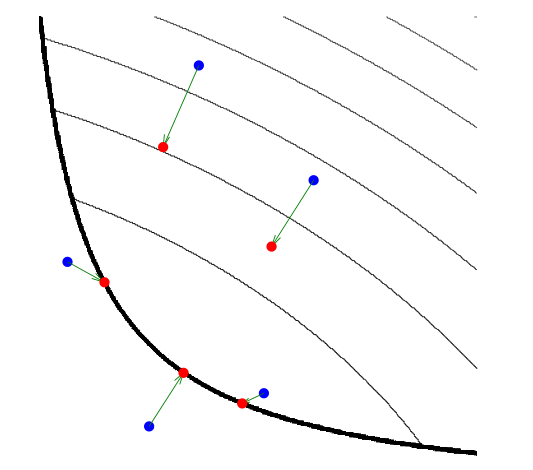
\includegraphics[width=0.75\linewidth]{img/proximal.png}
\caption{\label{fig:proximal}Illustration de l'opérateur proximal}
\end{figure}
}
\only<3>{
\begin{propriete}
Soit une fonction $f\in\Gamma_0(\RR^n)$. Alors, $\prox_f(x)$ existe et est unique pour tout $x\in\RR^n$.\\
De plus, il est caractérisé par : 
$$
\forall (x,p)\in \RR^n\times\RR^n\quad p=\prox_fx\quad\Longleftrightarrow\quad x-p\in\partial f(p)
$$
En particulier, si $f$ est différentiable alors : 
$$
\forall (x,p)\in \RR^n\times\RR^n\quad p=\prox_fx\quad \Longleftrightarrow \quad x-p=\nabla f(p)
$$
\end{propriete}
}
\only<4>{
\begin{propriete}
Le point $x^{\star}$ minimise $f$ si et seulement si 
$$
x^{\star} = \prox_f(x^{\star})
$$
\end{propriete} 
}
  \end{frame}
  \begin{frame}\frametitle{Algorithme de Douglas Rachford}
  \only<1>{
  \fbox{
  \parbox{\textwidth}{
  Soient $f_1$ et $f_2$ deux fonctions de $\Gamma_0(\RR^n)$ telles que $f_1+f_2\in\Gamma_0(\RR^n)$, en particulier le support de $f_1+f_2$ est non vide. Supposons que
  $$
  \lim_{\|x\|\rightarrow+\infty} f_1(x)+f_2(x) =+\infty
  $$
Considérons alors le problème de minimisation, 
Trouver $x\in\RR^n$ qui réalise le 
\begin{align}
\min_{x\in\RR^n}f_1(x)+f_2(x)
\label{eq:pbmminimi}
\end{align}
  }
}
}
\only<2>{
\begin{propriete}
Le problème \ref{eq:pbmminimi} admet une solution et pour tout $\gamma >0$, elle est caractérisée par :
$$
\left\{
\begin{array}{rcl}
x^{\star} &= & \prox_{\gamma f_2} y \\
\prox_{\gamma f_2}y &= & \prox_{\gamma f_1}(2\prox_{\gamma f_2}y -y)
\end{array}
\right.
$$
\end{propriete}
}
\only<3>{
\fbox{
  \parbox{\textwidth}{
\begin{align*}
&\text{Soient } \gamma >0 \text{ et } y_0\in \RR^n \\
&\text{Pour } n = 0,1,\ldots \\
&\quad x_n = \prox_{\gamma f_2} y_n\\
&\quad \lambda_n \in ]0,2[ \\
&\quad y_{n+1} = y_n + \lambda_n(\prox_{\gamma f_1} (2x_n-y_n)-x_n)\\
&\text{Fin}
\end{align*}
}
}
}
  \end{frame}
  
  \section{Résolution numérique}
\begin{frame}\frametitle{Problème}
Posons le changement de variable $m=fv$. 
	\begin{align*}
	\min_{(f,m)\in\mathcal{C}_v}\int_{[0,1]^n}\int_0^1 \frac{\|m(t,x)\|^2}{f(t,x)}dtdx
	\end{align*}
Avec,
	\begin{align*}
	C_v=&\{(f,m)\ |\ \frac{\partial f}{\partial t} + \text{div}_x (m) =0,\\
	&f(0,\cdot) = f_0,\ f(1,\cdot)=f_1,\\
	&m(\cdot,0) = m(\cdot,1)=0 \}
	\end{align*}
\end{frame}
\begin{frame}\frametitle{Grilles de discrétisations}
\only<1>{
\begin{figure}
\centering
	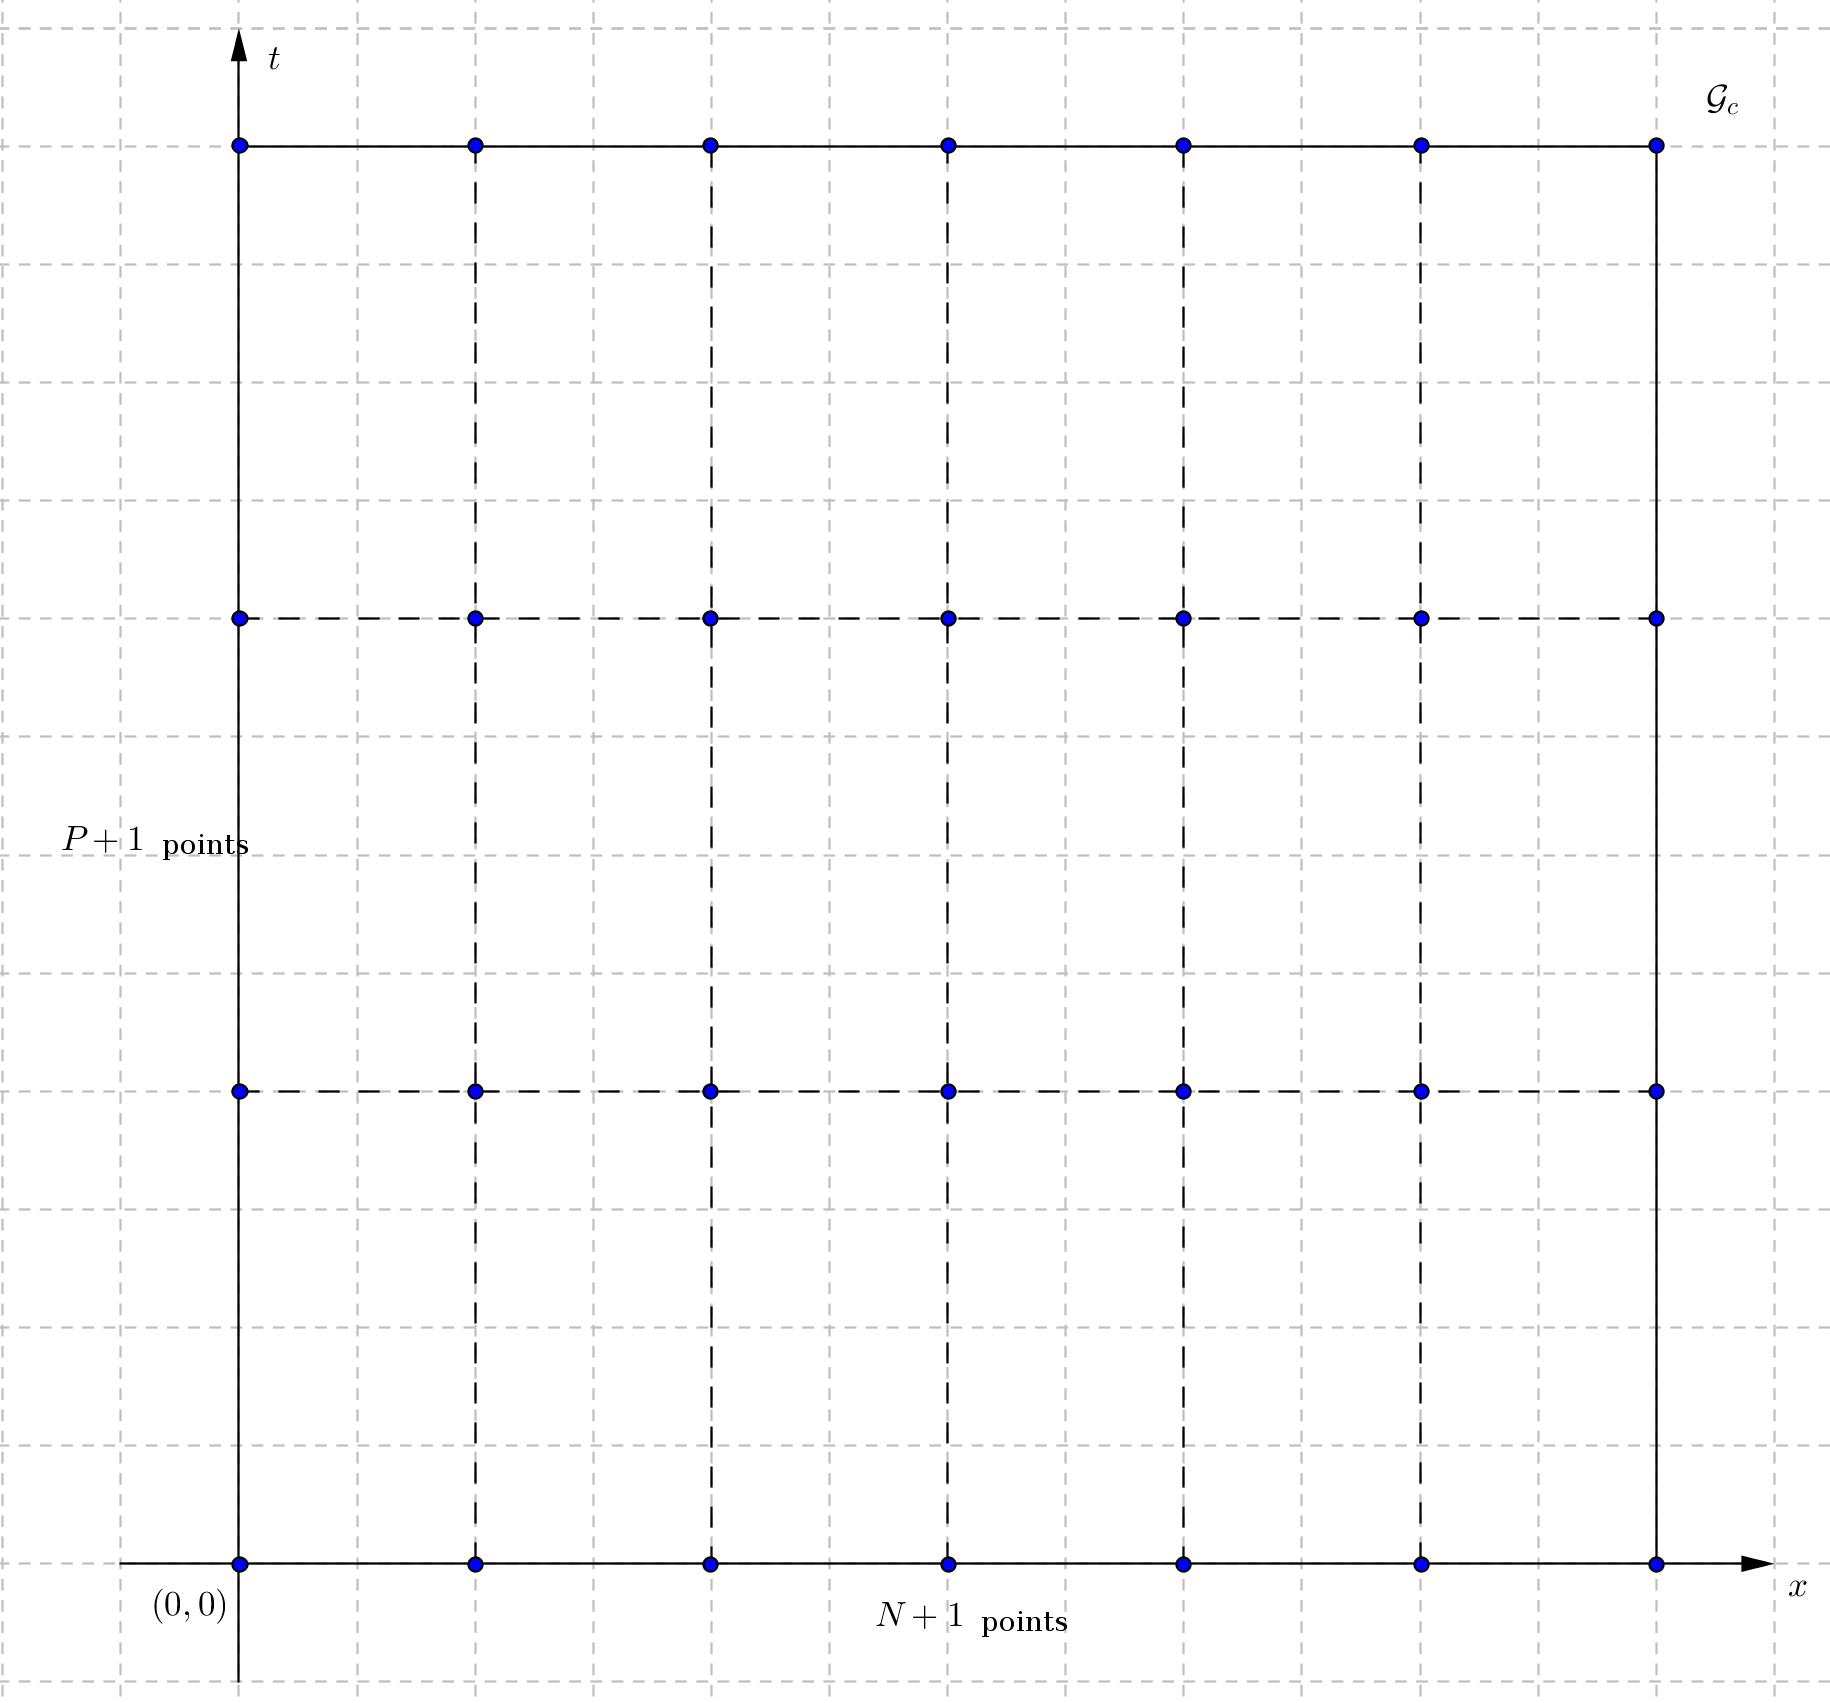
\includegraphics[width=0.7\linewidth]{img/grille_centree.png}
	\caption{Grille centrée}
	\label{fig:centered}
\end{figure}
}
\only<2>{
\begin{figure}[!h]
\centering
	\begin{subfigure}[b]{0.45\linewidth}
	\centering
	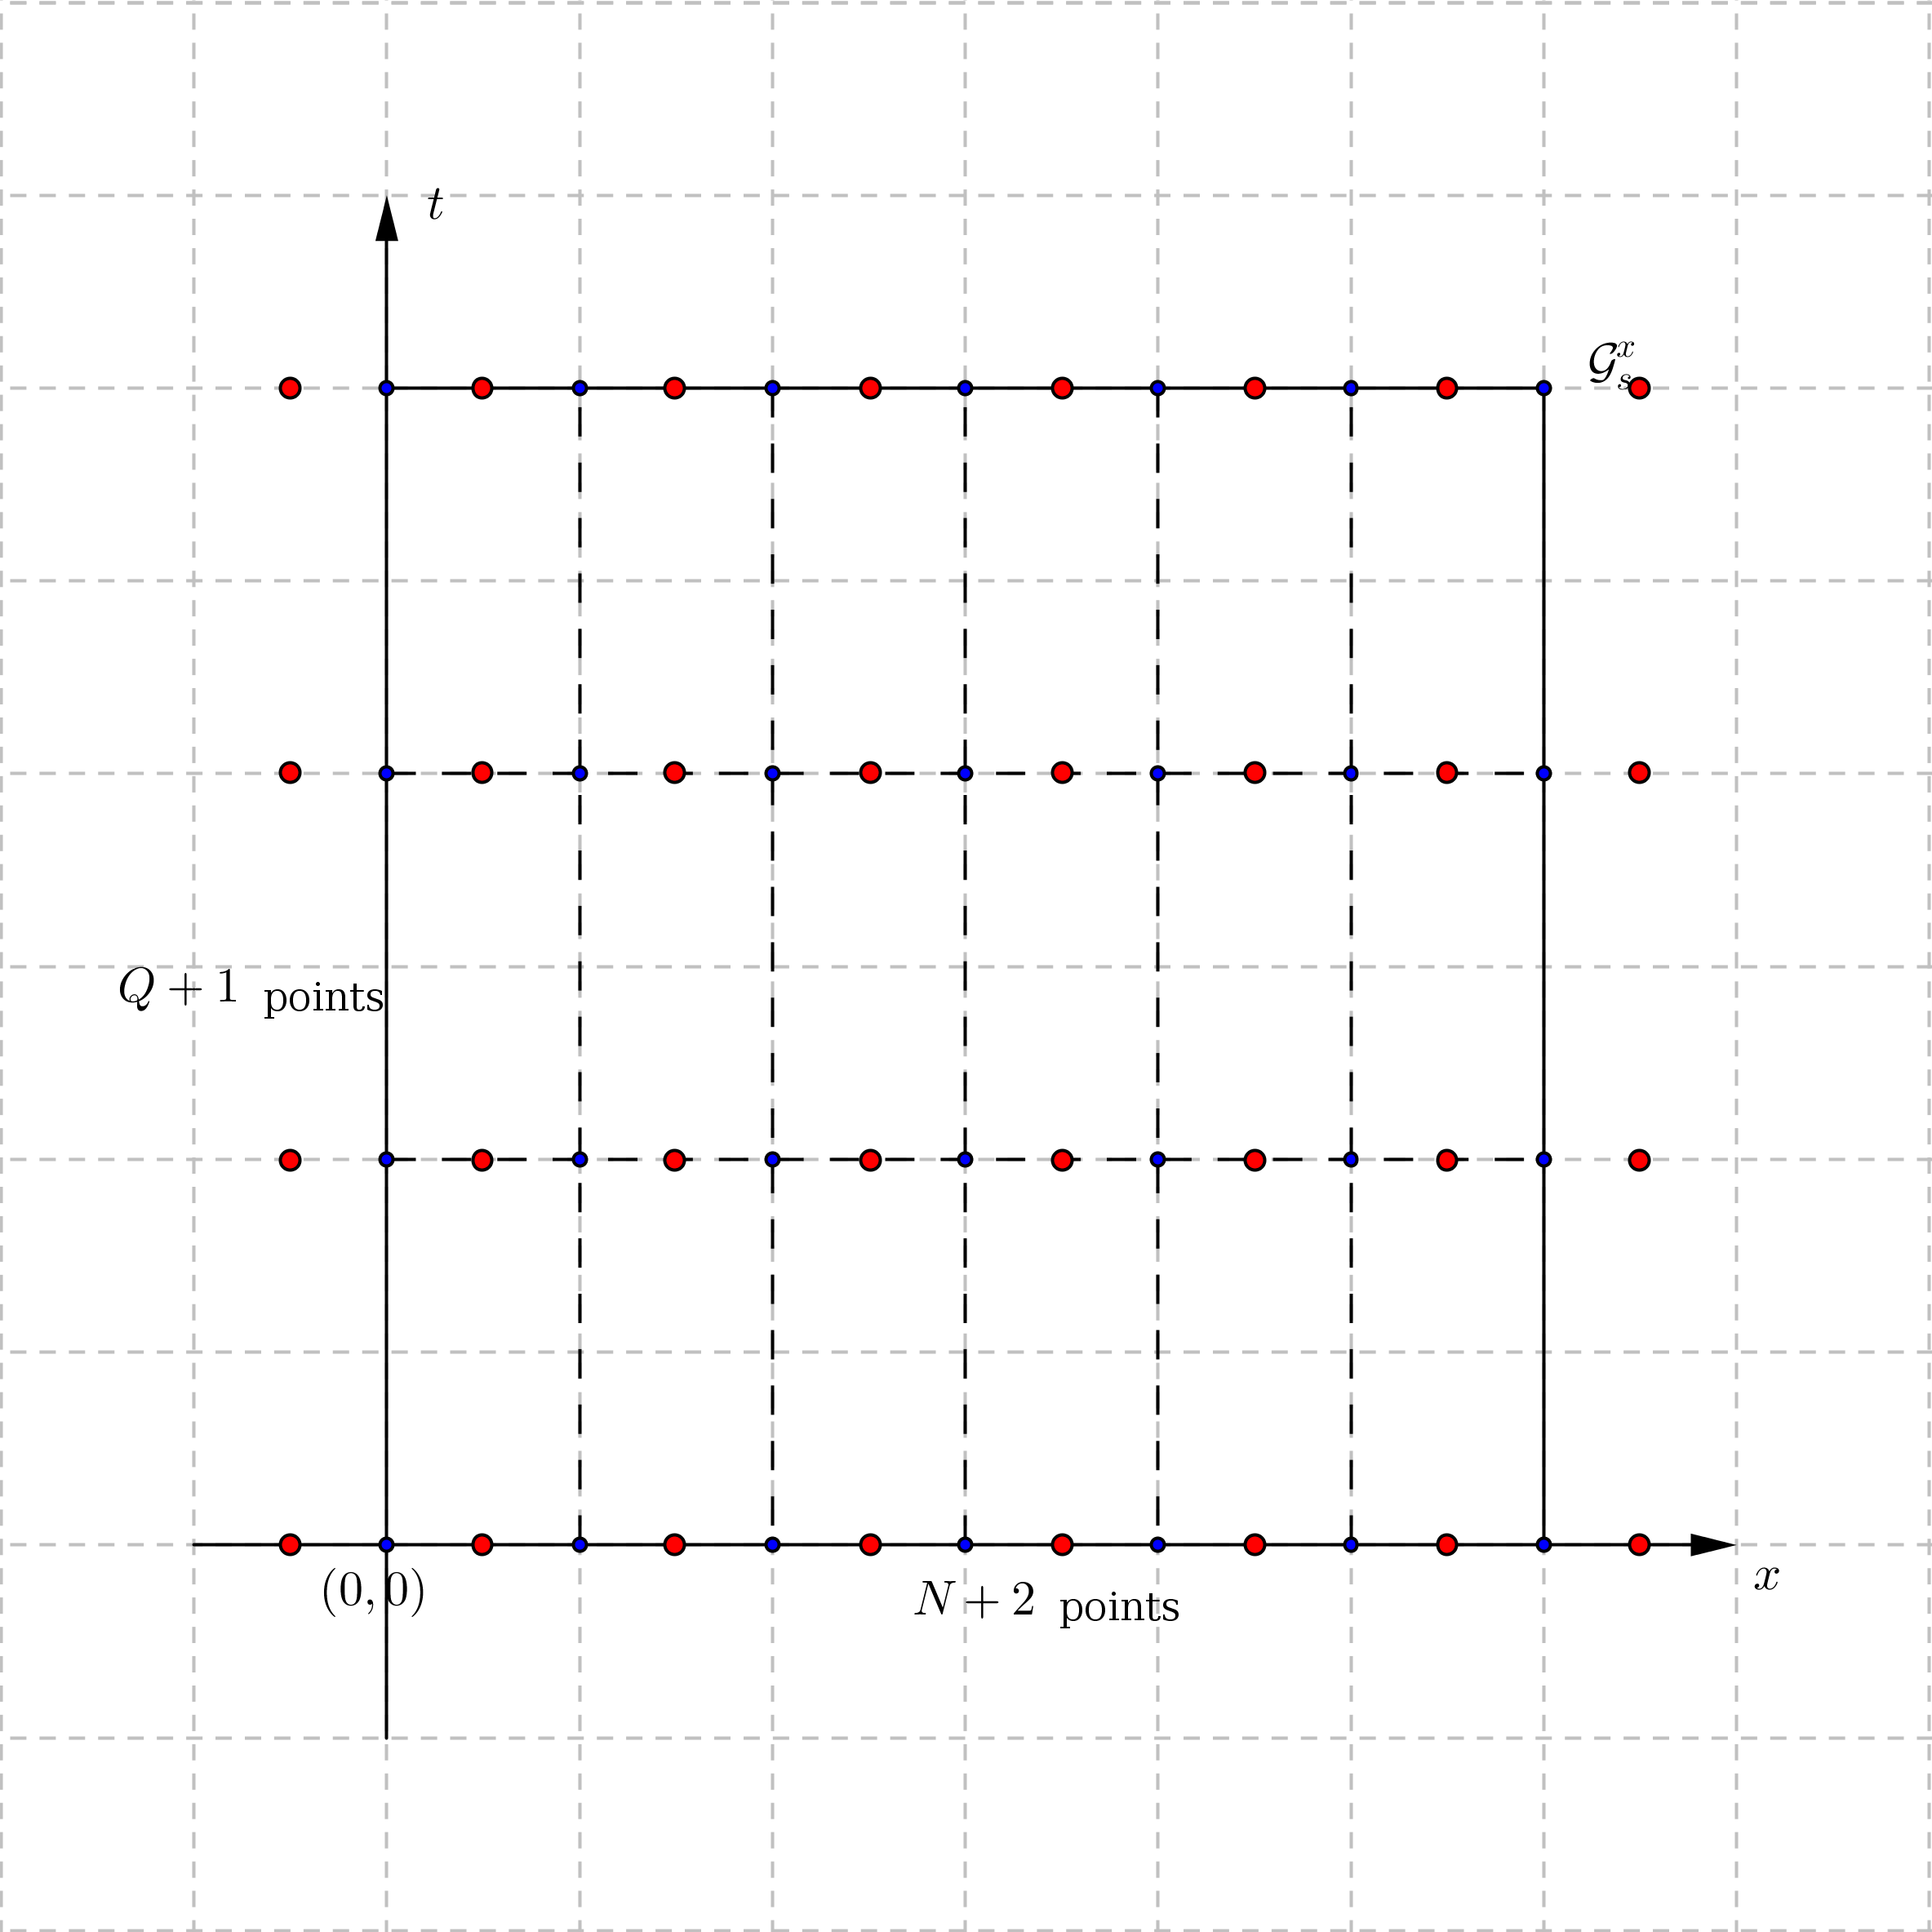
\includegraphics[width=0.9\linewidth]{img/grille_decentree_x.png}
	\caption{Grille décentrée en espace}
	\label{fig:staggeredX}
	\end{subfigure}
	~
	\begin{subfigure}[b]{0.45\linewidth}
	\centering
	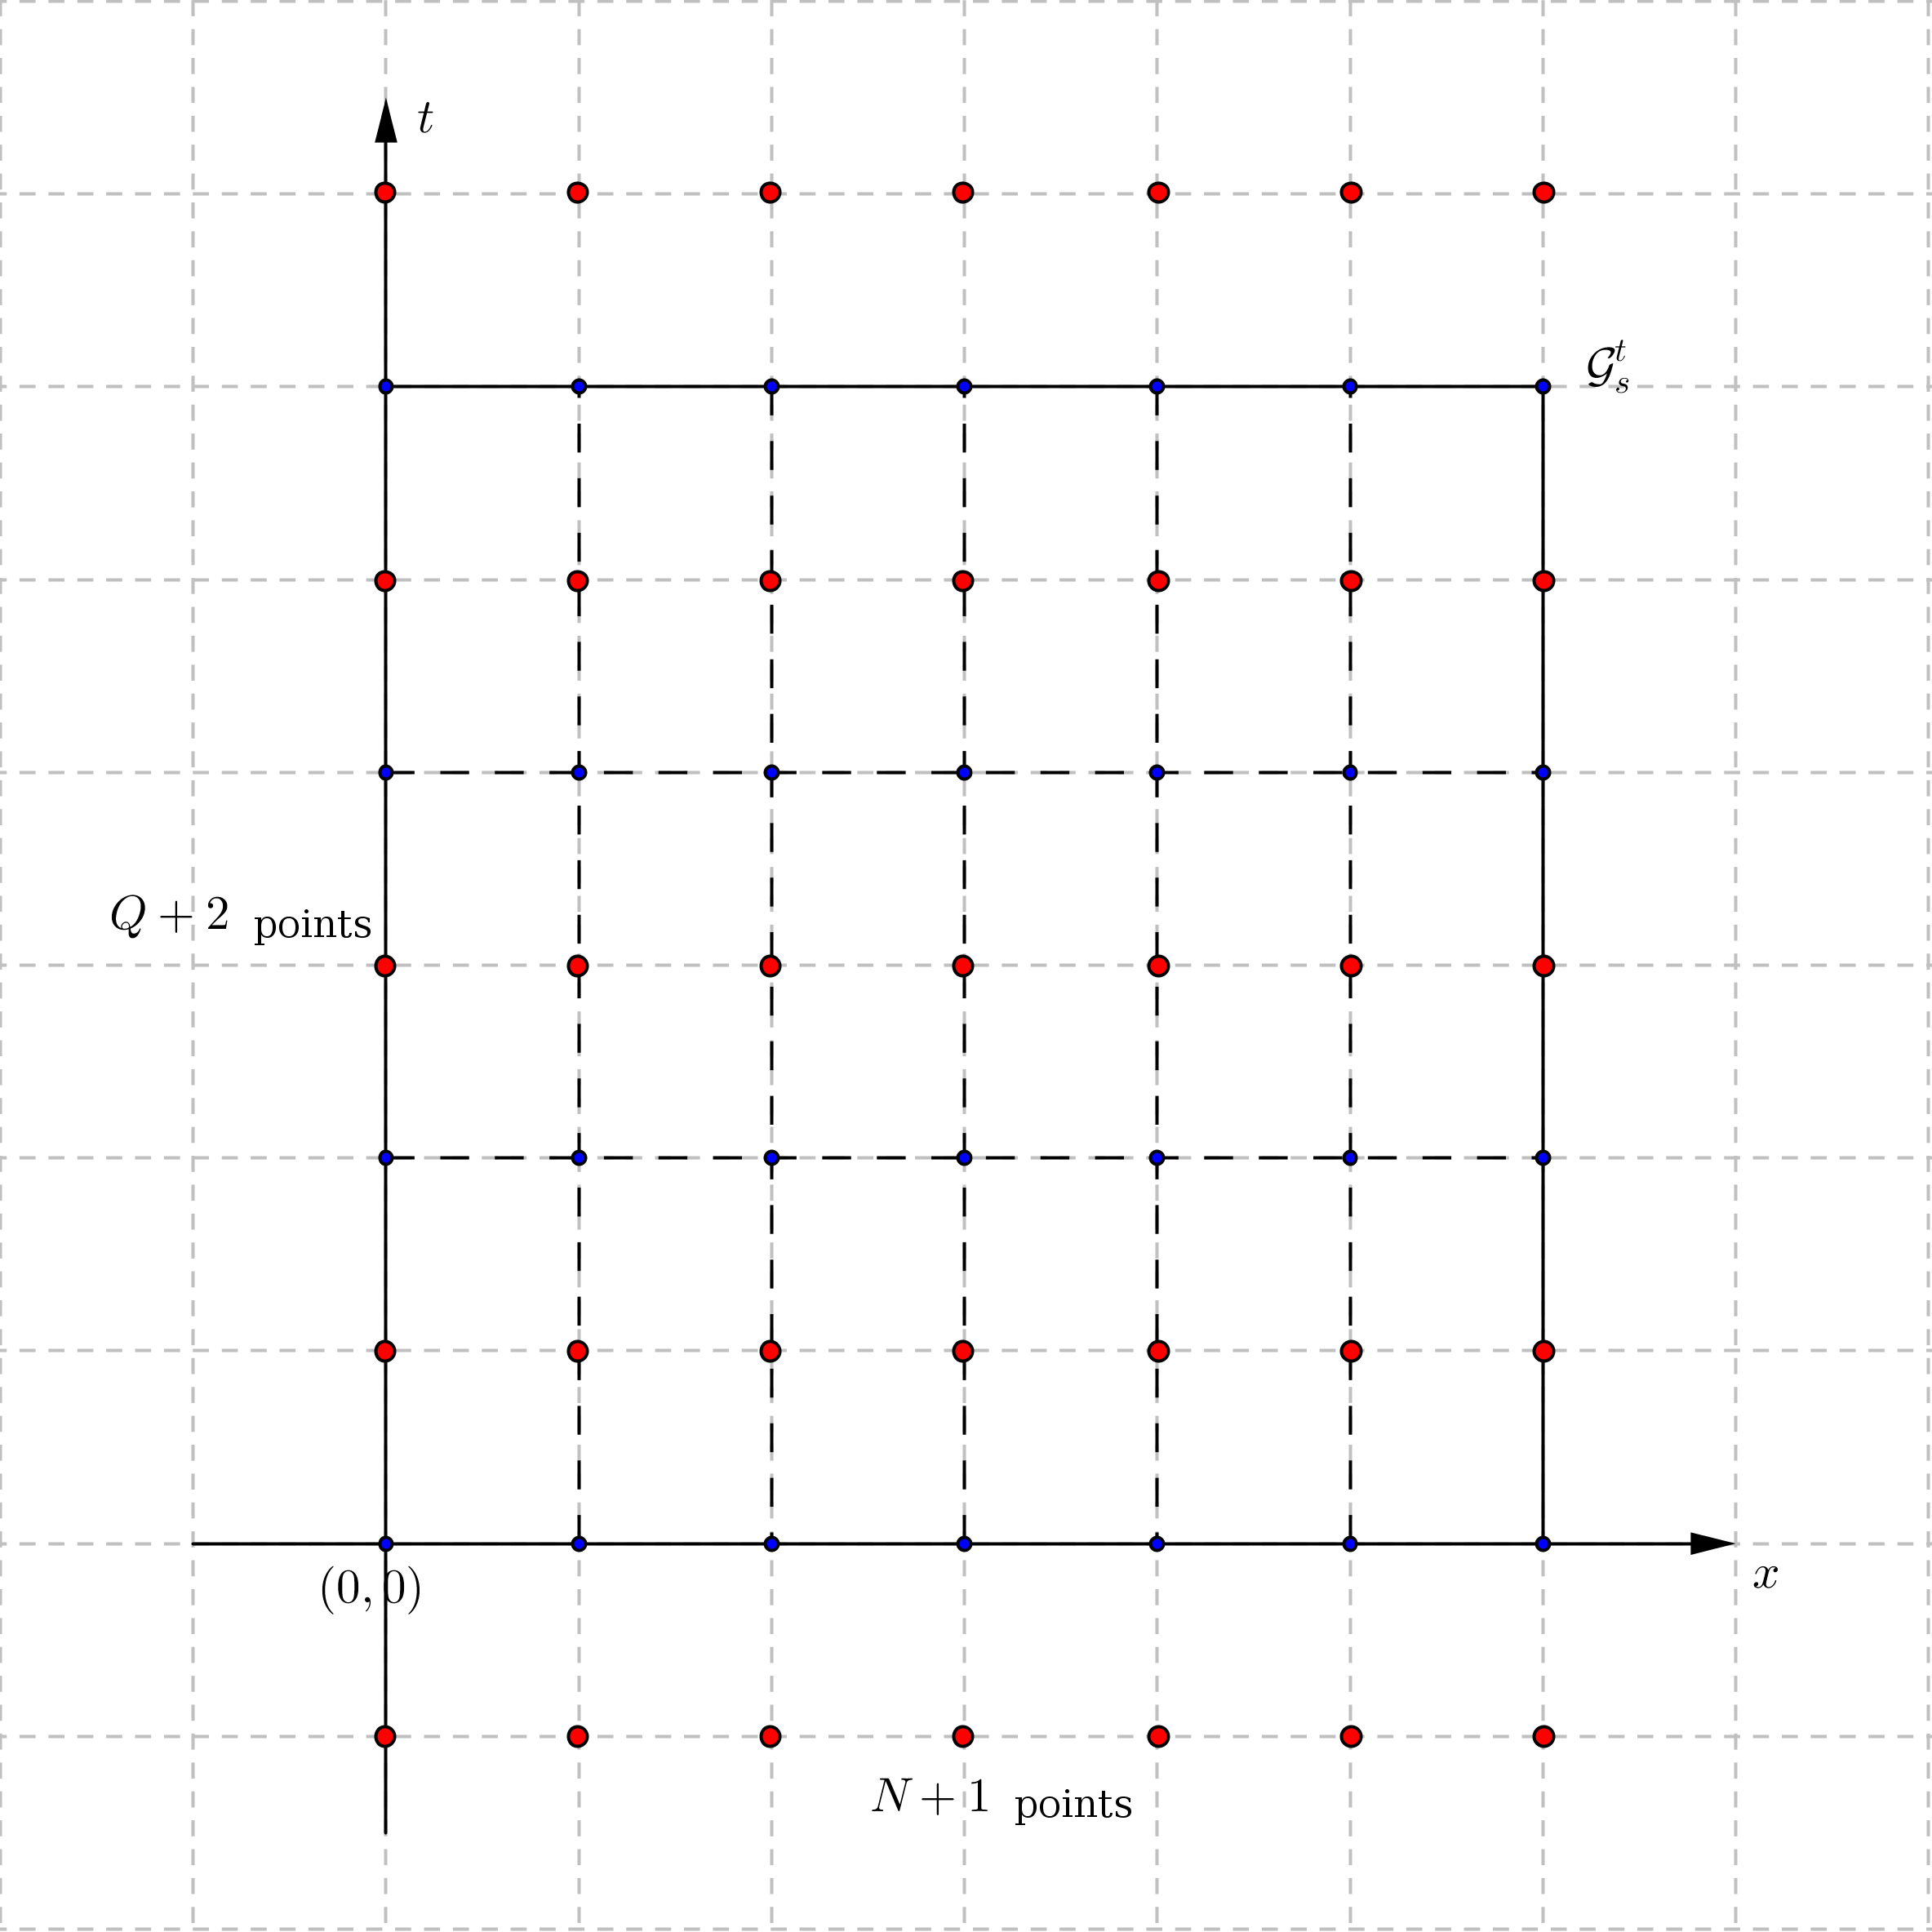
\includegraphics[width=0.9\linewidth]{img/grille_decentree_t.png}
	\caption{Grille décentrée en temps}
	\label{fig:staggeredT}
	\end{subfigure}
	\caption{Grilles de discrétisation pour $N=6$ et $Q=3$}
\end{figure}
}
\only<3>{
Notons $$
V = (m_{ij},f_{ij})_{0\leq i\leq N}^{0\leq j\leq Q}
$$ et 
$$U=(\bar{m},\bar{f})=\left((\bar{m}_{ij})_{-1\leq i\leq N}^{0\leq j\leq Q}, (\bar{f}_{ij})_{0\leq i\leq N}^{-1\leq j\leq Q}\right)$$
}
\end{frame}
  
  \begin{frame}\frametitle{Opérateurs discrétisés}
\only<1>{ Interpolation :
\begin{align*}
\fonction{\mathcal{I}}{\mathcal{E}_s}{\mathcal{E}_c}{(\bar{m},\bar{f})}{\left\{
\begin{array}{ccccc}
m_{i,j} &=& (\bar{m}_{i-1,j} &+& \bar{m}_{i,j})/2 \\
f_{i,j} &=& (\bar{f}_{i,j-1} &+& \bar{f}_{i,j})/2 \\
\end{array}
\right.
}
\end{align*}
}
\only<2>{Opérateur de divergence :
\begin{align*}
\fonction{\div}{\mathcal{E}_s}{\RR^{\mathcal{G}_c}}{U}{\div(U)_{i,j} = N(\bar{m}_{i,j} - \bar{m}_{i-1,j}) + Q(\bar{f}_{i,j} - \bar{f}_{i,j-1})
}
\end{align*}
}
\only<3>{Extraction des frontières
\begin{align*}
\fonction{b}{\mathcal{E}_s}{\RR^{Q+1}\times\RR^{Q+1}\times\RR^{N+1}\times\RR^{N+1}}{U}{\left( (\bar{m}_{-1,j},\bar{m}_{N,j})_{j=0}^Q,(\bar{f}_{i,-1},\bar{f}_{i,Q})_{i=0}^N \right)}
\end{align*}
}  
  \end{frame}
  
  \begin{frame}\frametitle{Problème discrétisé}
  \begin{align*}
	\min_{(U,V)\in\mathcal{E}_s\times\mathcal{E}_c} \mathcal{J}(V) + \iota_{\mathcal{C}}(U) + \iota_{\mathcal{C}_s}(U,V)
	\end{align*}

Ici, l'indicatrice d'un ensemble convexe est définie de la façon suivante ; $ \iota_{\mathcal{C}}=\left\{\begin{array}{cl}
0 &\text{si } U\in\mathcal{C} \\
+\infty &\text{sinon }
\end{array}\right.$.\\

	\begin{align*}
	\mathcal{J}(V) &= \sum_{k\in\mathcal{G}_c} \frac{\|m_k\|^2}{f_k}\\
	\mathcal{C}  &= \left\{ U\in \mathcal{E}_s\ |\ \div(U)=0,\ b(U) = b_0 = \left( 0,0,f_0,f_1\right) \right\} \\
	\mathcal{C}_s&=\left\{(U,V)\in\mathcal{E}_s\times\mathcal{E}_c\ |\ V=\mathcal{I}(U)\right\}
	\end{align*}
  \end{frame}
  
\begin{frame}\frametitle{Algorithme de Douglas Rachford pour le problème de transport optimal}
\begin{align*}
\prox_{\gamma f_1}(U,V) & = \left(\proj_{\mathcal{C}}(U),\prox_{\gamma \mathcal{J}}(V) \right) \\
\prox_{\gamma f_2}(U,V) & = \proj_{\mathcal{C}_s}(U,V)
\end{align*}

\fbox{
  \parbox{\textwidth}{
 	Soit une suite $(x_n,y_n)\in\left(\mathcal{E}_s\times\mathcal{E}_c\right)^2$. A partir, d'une condition initiale $y_0$, 
 	
 	\begin{equation*}
 		\begin{aligned}
 			x_n &= \proj_{\mathcal{C}_s}(y_n) \\
 		y_{n+1} &= y_n + \lambda_n \left(\prox_{\gamma f_1}(2x_n-y_n)-x_n\right) \\
 		\end{aligned}
 	\end{equation*}
 	
 	Alors $x_n\rightarrow x^{\star}$ une solution du problème. 
  }
}
\end{frame}  
  
\begin{frame}\frametitle{Opérateur proximal de la fonction de coût}
\begin{proposition}
\label{prop:proxJ}
Nous avons
\begin{align*}
\forall w\in\mathcal{G},\ \prox_{\gamma \mathcal{J}}(w) = \left( \prox_{\gamma J}(w_k)\right)_{k\in\mathcal{G}}
\end{align*}
Où, pour tout $w_k=(m_k,f_k)\in\RR^n\times\RR$, 
$$
\prox_{\gamma J}(m_k,f_k) =\left\{
\begin{array}{cl}
\left(\frac{f^{\star}_k m_k}{f^{\star}_k+\gamma} ,f^{\star}_k\right) & \text{ si } f^{\star}_k >0\\
(0,0) & \text{ sinon }
\end{array}\right.
$$
et $f^{\star}_k$ est la plus grande racine réelle du polynôme de degré 3 : 
\begin{align}
P(X) = (X-f_k)(X+\gamma)^2 -\frac{\gamma}{2}\|m_k\|^2=0
\end{align}
\end{proposition}
\end{frame}	  

\begin{frame}\frametitle{Projection sur $\mathcal{C}$}
Écrivons,
\begin{align*}
\mathcal{C}=\left\{U\in\mathcal{E}_s\ |\ AU=y\right\} \quad A=\begin{pmatrix}
\div \\
b
\end{pmatrix},\ y=\begin{pmatrix}
0 \\
b_0
\end{pmatrix}
\end{align*}
C'est la projection sur un ensemble convexe sous contraintes. 
\begin{align*}
\proj_{\mathcal{C}}(U) = U - A^{\star} (AA^{\star})^{-1}(y-AU)
\end{align*}
\end{frame}
  
\begin{frame}\frametitle{Projection sur $\mathcal{C}_s$}
$$
\mathcal{C}_s=\left\{(U,V)\in\mathcal{E}_s\times\mathcal{E}_c\ |\ V=\mathcal{I}(U)\right\}
$$
\begin{align*}
\proj_{\mathcal{C}_s}(U,V) &= (\tilde{U},\mathcal{I}(\tilde{U}))\\
&\tilde{U}= (Id+\mathcal{I}^{\star}\mathcal{I})^{-1}(U+\mathcal{I}^{\star}(V))
\end{align*}
\end{frame}

\begin{frame}\frametitle{Coût généralisé}
\only<1>{
\begin{align}
\min_{U\in\mathcal{E}_s}\mathcal{J}_{\omega}^{\beta}(\mathcal{I}(U))+\iota_{\mathcal{C}}(U)
\end{align}
Où, $\beta\in[0,1]$, et le vecteur de poids $\omega=(\omega_k)_{k\in\mathcal{G}_c}$ vérifie $1\leq \omega_k\leq +\infty$. La fonctionnelle généralisée est définie par : 
\begin{align}
\mathcal{J}_{\omega}^{\beta}(V) &= \sum_{k\in\mathcal{G}_c} \omega_kJ_{\beta}(m_k,f_k)\\
\forall (m,f)\in\RR\times\RR,\quad &J_{\beta}=\left\{ \begin{array}{cl}
\frac{\|m\|^2}{2f^{\beta}} & \text{si } f>0 \\
0 &\text{si } (m,f) = (0,0)\\
+\infty & \text{sinon} 
\end{array}\right.
\end{align}
}
\only<2>{
\remarques{
\begin{enumerate}
\item Le coefficient $\beta\in[0,1]$ agit comme un interrupteur entre l'interpolation $L^2$ ($\beta =0$) entre les deux densités et le calcul du transport optimal ($\beta =1$), i.e. le calcul de la distance $L^2$ de Wasserstein.
\item Les poids $\omega_k$ pondèrent certaines régions de l'espace temps et permettent d'autoriser plus au moins le passage d'une densité dans une région de l'espace ; $\omega_k=+\infty$ correspond à une zone interdite. 
\end{enumerate}}
}
\end{frame}
\section{Exemple numériques}
\subsection{Exemple 1D}
\begin{frame}%\frametitle{Exemple 1D}
\begin{figure}[!h]
\centering 
	\begin{subfigure}[b]{0.48\linewidth}
	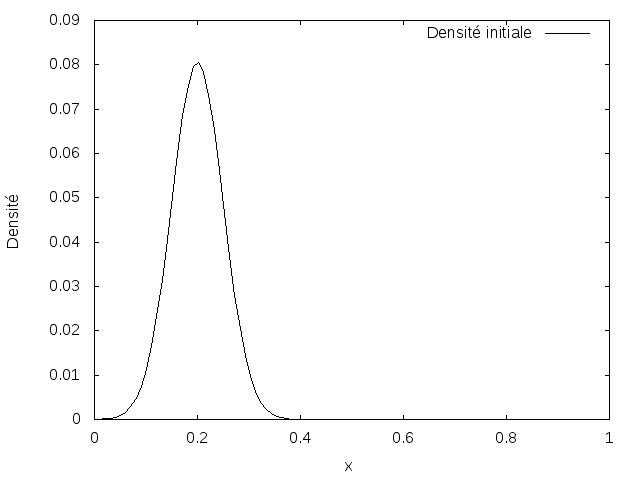
\includegraphics[width=\textwidth]{img/1DGaussian100x100/f0.png}
	\caption{Densité initiale}
	\end{subfigure}
	~
	\begin{subfigure}[b]{0.48\linewidth}
	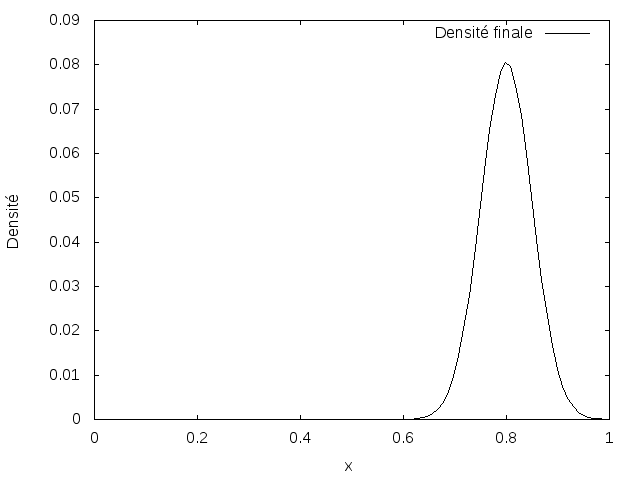
\includegraphics[width=\textwidth]{img/1DGaussian100x100/f1.png}
	\caption{Densité finale}
	\end{subfigure}
	
	\begin{subfigure}[b]{0.48\linewidth}
	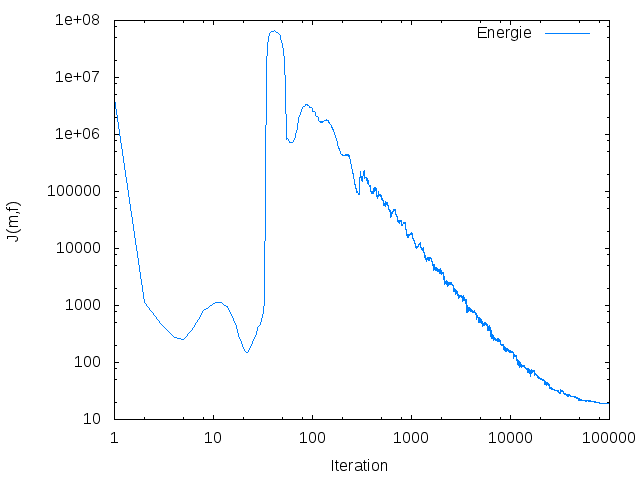
\includegraphics[width=\textwidth]{img/1DGaussian100x100/energie.png}
	\caption{$\mathcal{J}(m,f)$}
	\end{subfigure}
	~
	\begin{subfigure}[b]{0.48\linewidth}
	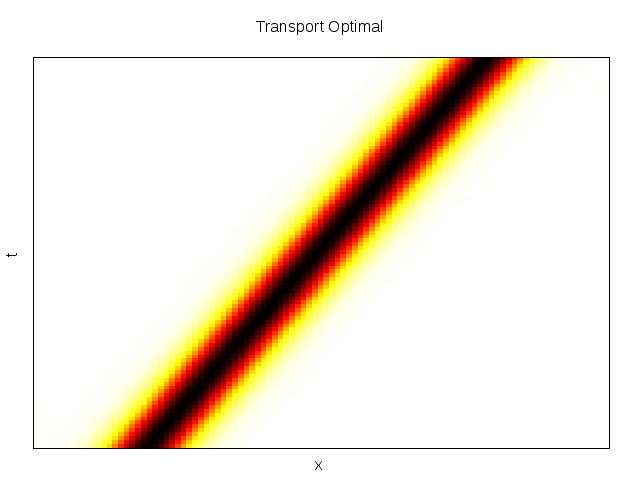
\includegraphics[width=\textwidth]{img/1DGaussian100x100/transport.png}
	\caption{Le Transport}
	\end{subfigure}	
	\caption{Données pour le transport de deux gaussiennes}
\end{figure}
\end{frame}

\begin{frame}
\begin{figure}[!h]
\centering 
	\begin{subfigure}[b]{0.48\linewidth}
	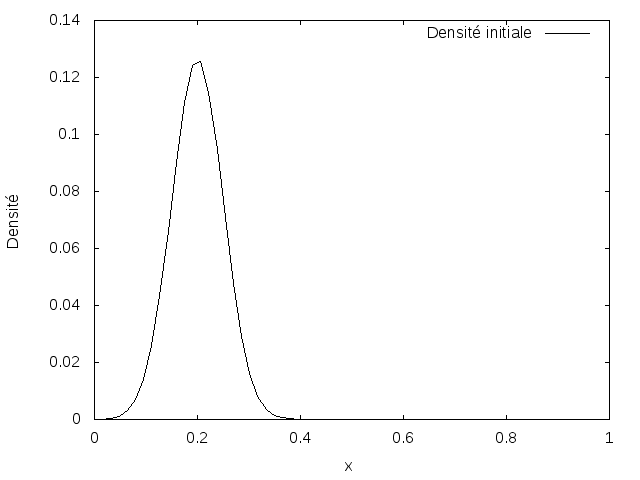
\includegraphics[width=\textwidth]{img/1DMixture/f0.png}
	\caption{Densité initiale}
	\end{subfigure}
	~
	\begin{subfigure}[b]{0.48\linewidth}
	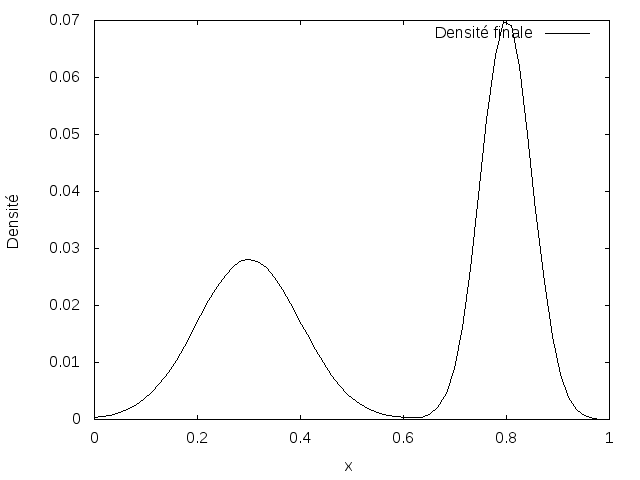
\includegraphics[width=\textwidth]{img/1DMixture/f1.png}
	\caption{Densité finale}
	\end{subfigure}
	
	\begin{subfigure}[b]{0.48\linewidth}
	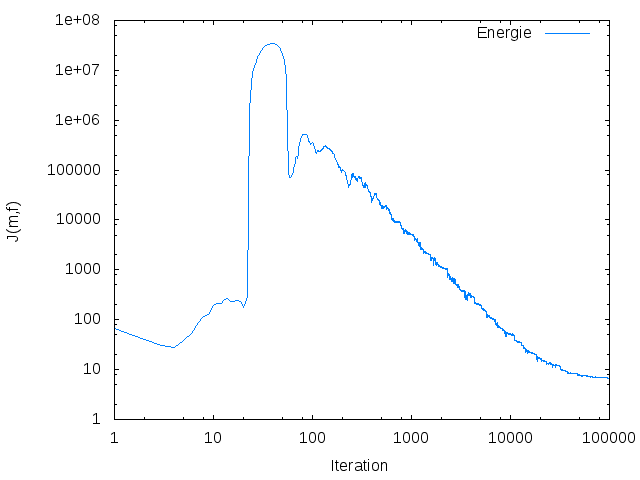
\includegraphics[width=\textwidth]{img/1DMixture/energie.png}
	\caption{$\mathcal{J}(m,f)$}
	\end{subfigure}
	~
	\begin{subfigure}[b]{0.48\linewidth}
	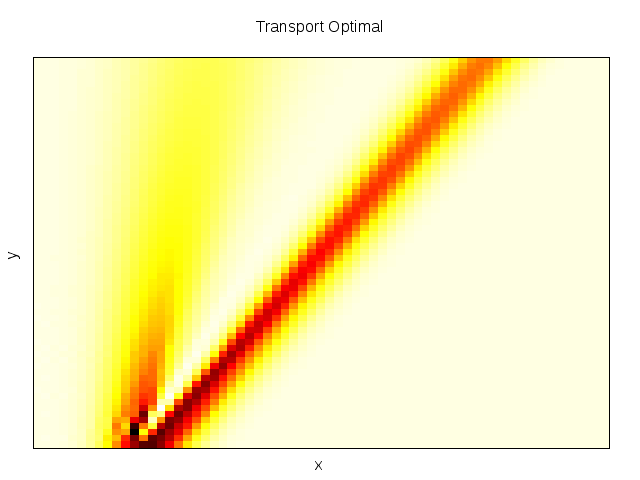
\includegraphics[width=\textwidth]{img/1DMixture/transport.png}
	\caption{Le Transport}
	\end{subfigure}	
	\caption{Données pour le transport d'une gaussienne sur deux gaussiennes}
\end{figure}
\end{frame}

\begin{frame}
\begin{figure}[!h]
\centering 
	\begin{subfigure}[b]{0.48\linewidth}
	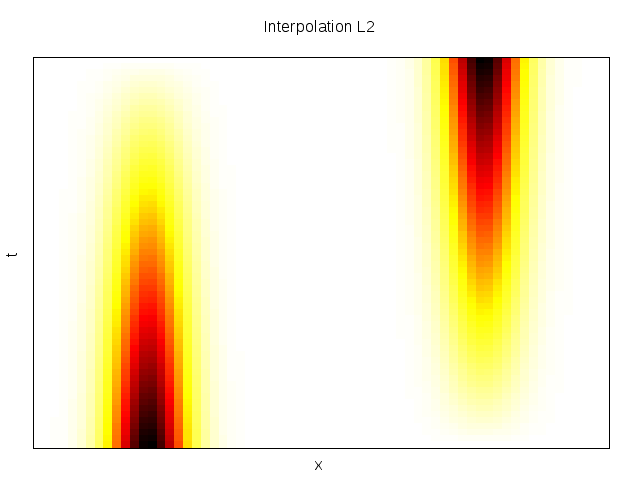
\includegraphics[width=\textwidth]{img/1DGeneralise/transport0.png}
	\caption{$\beta = 0$}
	\end{subfigure}
	~
	\begin{subfigure}[b]{0.48\linewidth}
	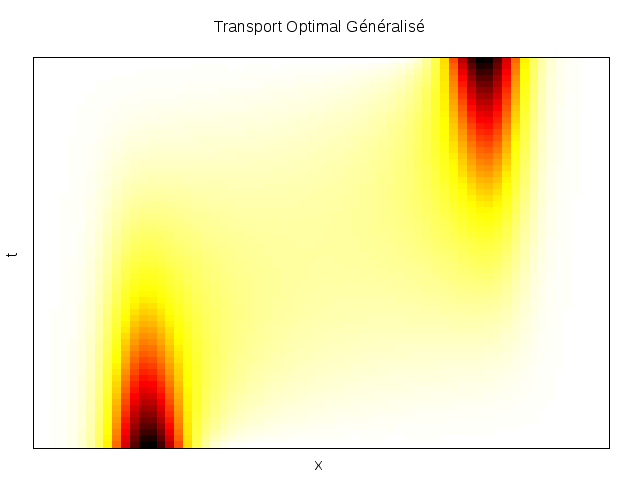
\includegraphics[width=\textwidth]{img/1DGeneralise/transport25.png}
	\caption{$\beta = 1/4$}
	\end{subfigure}	
	
	\begin{subfigure}[b]{0.48\linewidth}
	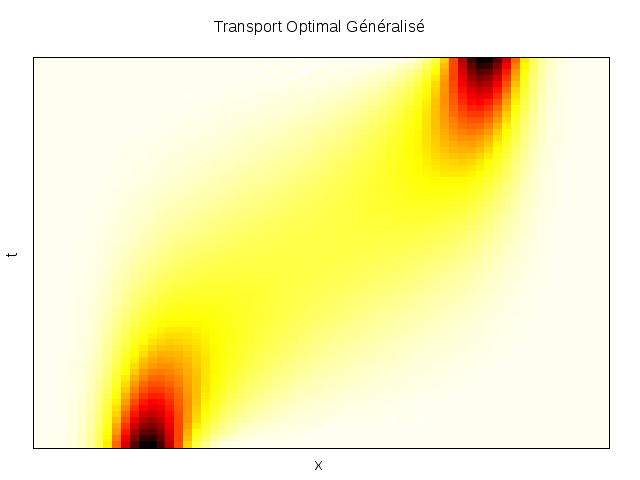
\includegraphics[width=\textwidth]{img/1DGeneralise/transport50.png}
	\caption{$\beta = 1/2$}
	\end{subfigure}
	~
	\begin{subfigure}[b]{0.48\linewidth}
	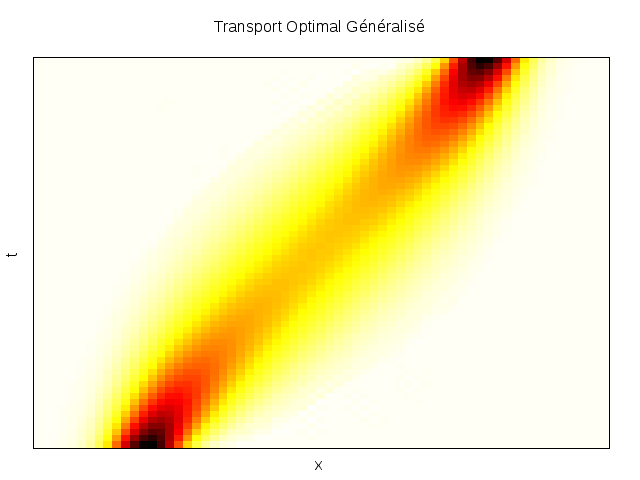
\includegraphics[width=\textwidth]{img/1DGeneralise/transport75.png}
	\caption{$\beta = 3/4$}
	\end{subfigure}	
\end{figure}
\end{frame}

\begin{frame}
\begin{figure}[!h]
\centering 
	\begin{subfigure}[b]{0.48\linewidth}
	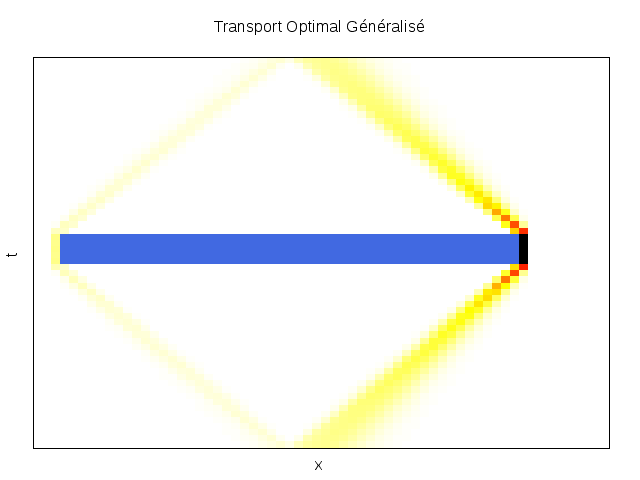
\includegraphics[width=\textwidth]{img/1DObstacle/resultat.png}
	\caption{Un obstacle au milieu du passage}
	\end{subfigure}
	~
	\begin{subfigure}[b]{0.48\linewidth}
	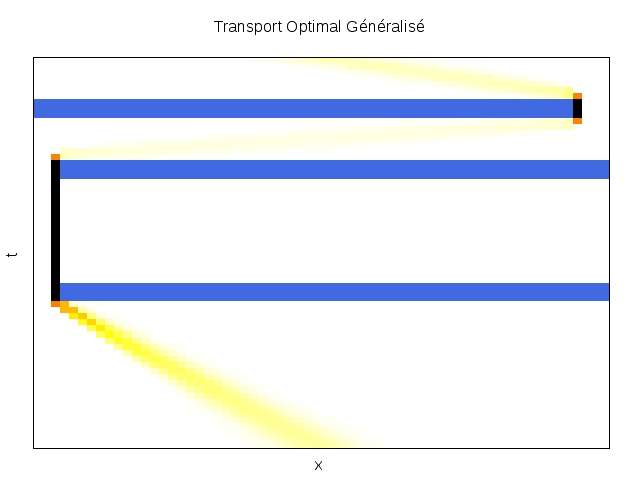
\includegraphics[width=\textwidth]{img/1DLabyrinthe/resultat.png}
	\caption{Un "labyrinthe"}
	\end{subfigure}	
	\caption{Transport de deux gaussienne avec des obstacles}
\end{figure}
\end{frame}

\subsection{Exemple 2D}
\begin{frame}
\begin{figure}[!h]
\centering 
\hspace{-0.5cm}
	\begin{subfigure}[b]{0.3\linewidth}
	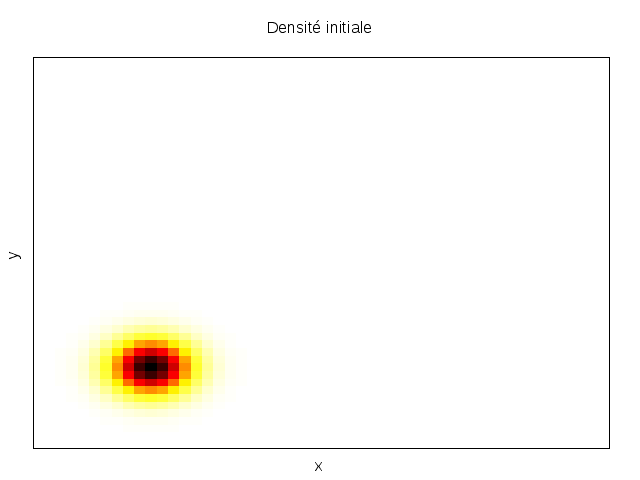
\includegraphics[width=\textwidth]{img/2DGaussian/f0.png}
	\caption{Densité initiale}
	\end{subfigure}
	~
	\begin{subfigure}[b]{0.3\linewidth}
	\includegraphics[width=\textwidth]{img/2DGaussian/f1.png}
	\caption{Densité finale}
	\end{subfigure}
	~
	\begin{subfigure}[b]{0.35\linewidth}
	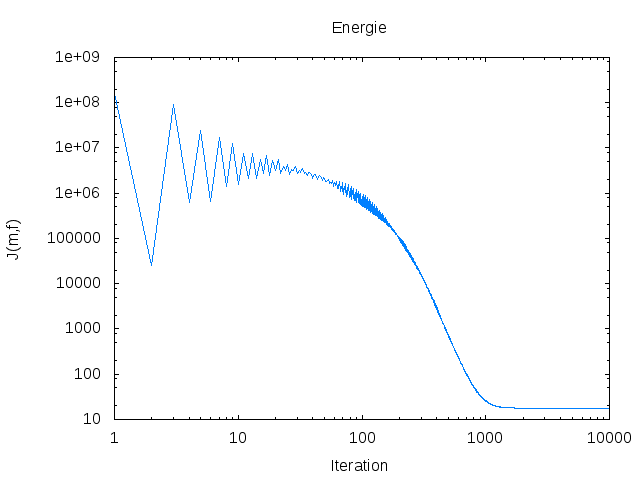
\includegraphics[width=\textwidth]{img/2DGaussian/energie.png}
	\caption{Energie}
	\end{subfigure}
	~
	
	\begin{subfigure}[b]{0.22\linewidth}
	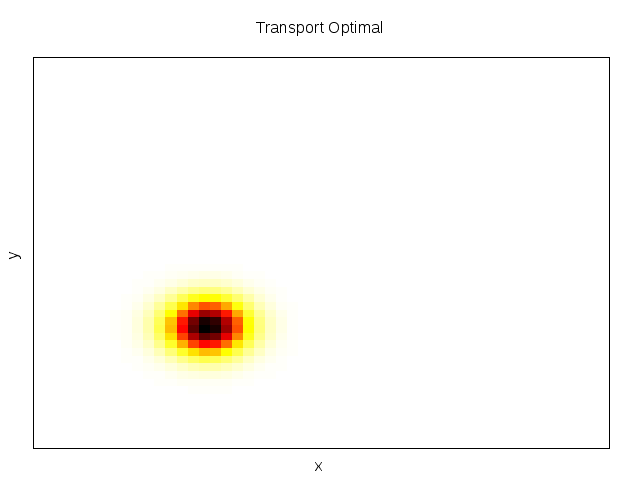
\includegraphics[width=\textwidth]{img/2DGaussian/C_00010.png}
	\caption{$t=0.2$}
	\end{subfigure}
	~
	\begin{subfigure}[b]{0.22\linewidth}
	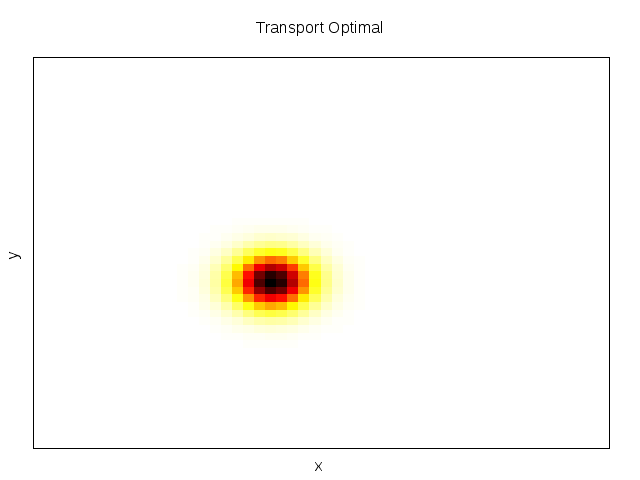
\includegraphics[width=\textwidth]{img/2DGaussian/C_00020.png}
	\caption{$t=0.4$}
	\end{subfigure}
	~
	\begin{subfigure}[b]{0.22\linewidth}
	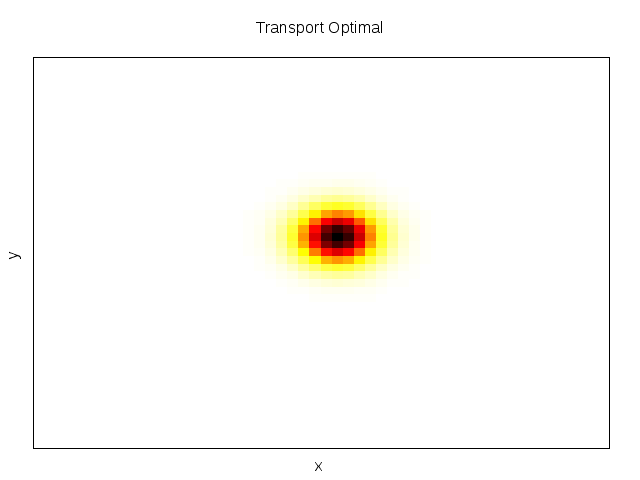
\includegraphics[width=\textwidth]{img/2DGaussian/C_00030.png}
	\caption{$t=0.6$}
	\end{subfigure}
	~
	\begin{subfigure}[b]{0.22\linewidth}
	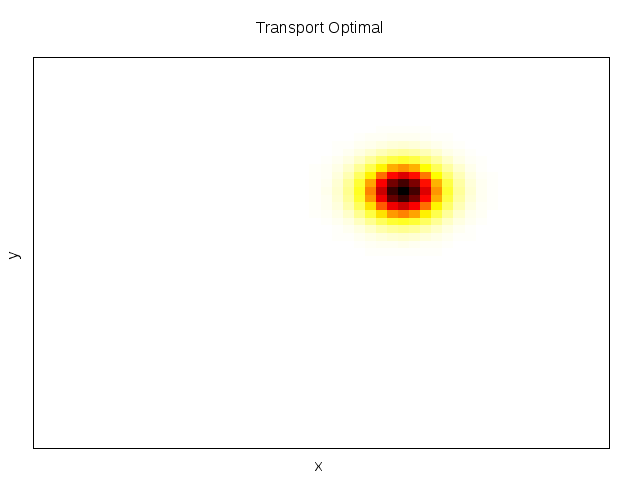
\includegraphics[width=\textwidth]{img/2DGaussian/C_00040.png}
	\caption{$t=0.8$}
	\end{subfigure}
	\caption{Transport de deux gaussienne $N=P=Q=50$}
\end{figure}
\end{frame}

\begin{frame}
\begin{figure}[!h]
\centering 
\hspace{-0.5cm}
	\begin{subfigure}[b]{0.3\linewidth}
	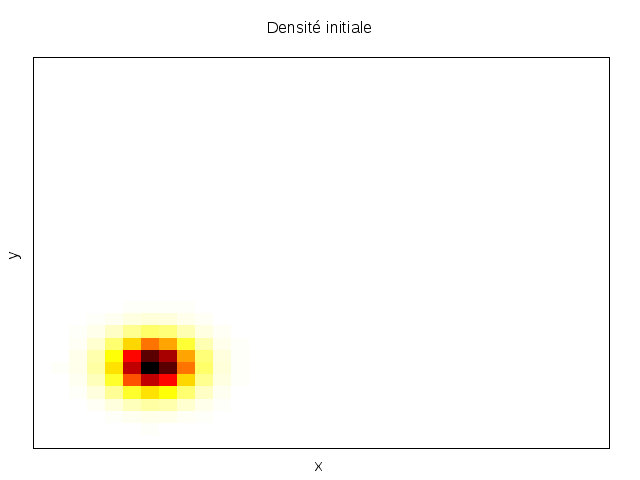
\includegraphics[width=\textwidth]{img/2DMixture/f0.png}
	\caption{Densité initiale}
	\end{subfigure}
	~
	\begin{subfigure}[b]{0.3\linewidth}
	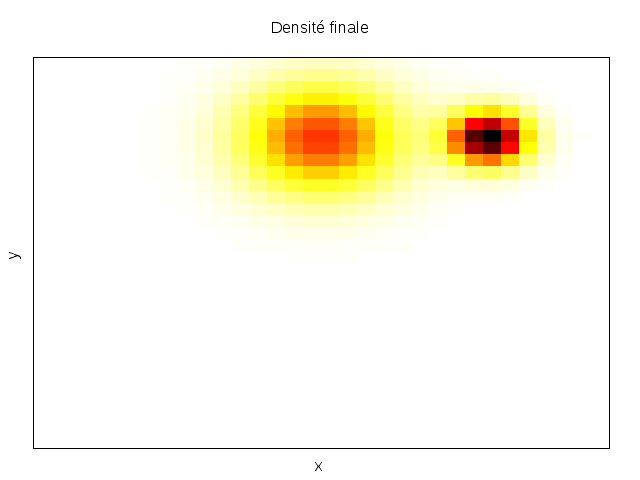
\includegraphics[width=\textwidth]{img/2DMixture/f1.png}
	\caption{Densité finale}
	\end{subfigure}
	~
	\begin{subfigure}[b]{0.35\linewidth}
	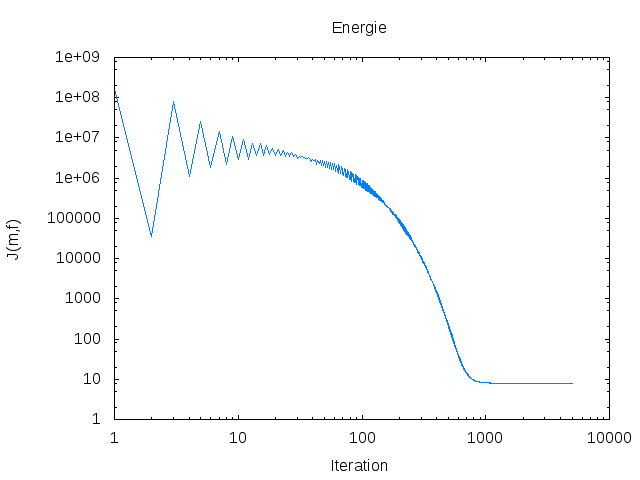
\includegraphics[width=\textwidth]{img/2DMixture/energie.png}
	\caption{Energie}
	\end{subfigure}
	~
	
	\begin{subfigure}[b]{0.22\linewidth}
	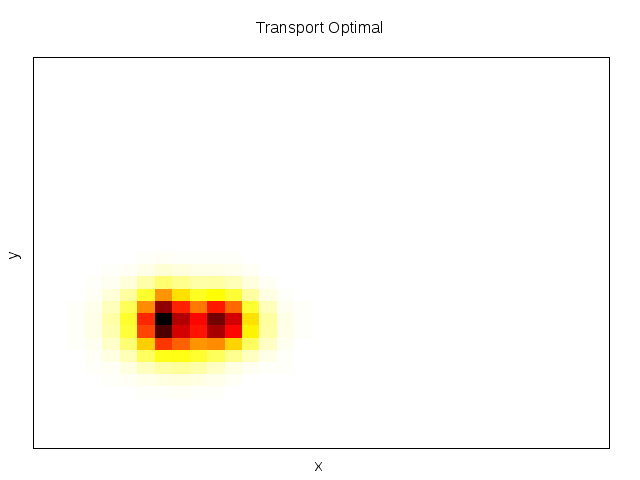
\includegraphics[width=\textwidth]{img/2DMixture/C_00007.png}
	\caption{$t=0.2$}
	\end{subfigure}
	~
	\begin{subfigure}[b]{0.22\linewidth}
	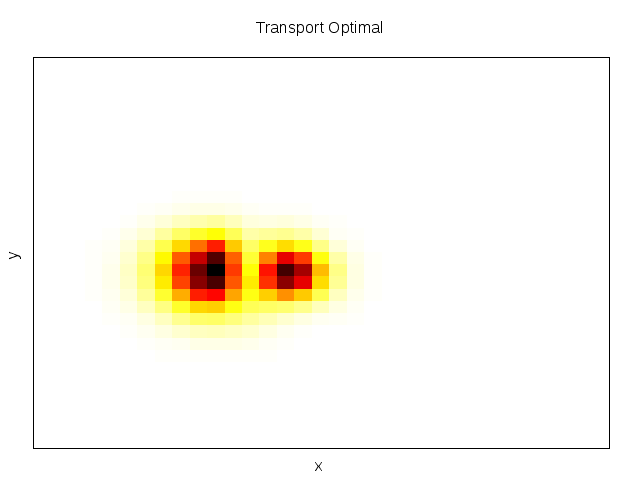
\includegraphics[width=\textwidth]{img/2DMixture/C_00014.png}
	\caption{$t=0.4$}
	\end{subfigure}
	~
	\begin{subfigure}[b]{0.22\linewidth}
	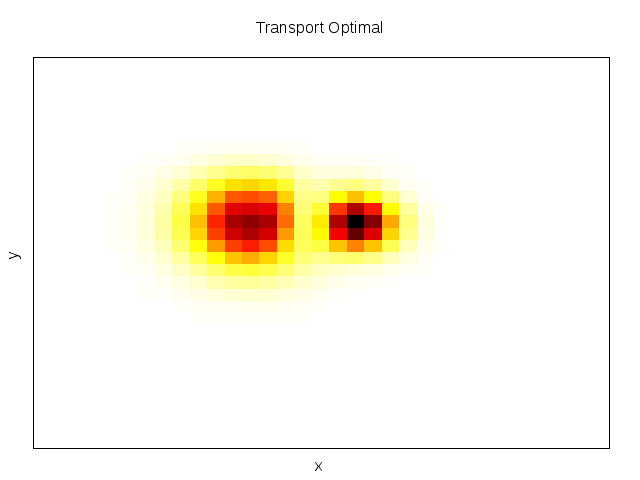
\includegraphics[width=\textwidth]{img/2DMixture/C_00021.png}
	\caption{$t=0.6$}
	\end{subfigure}
	~
	\begin{subfigure}[b]{0.22\linewidth}
	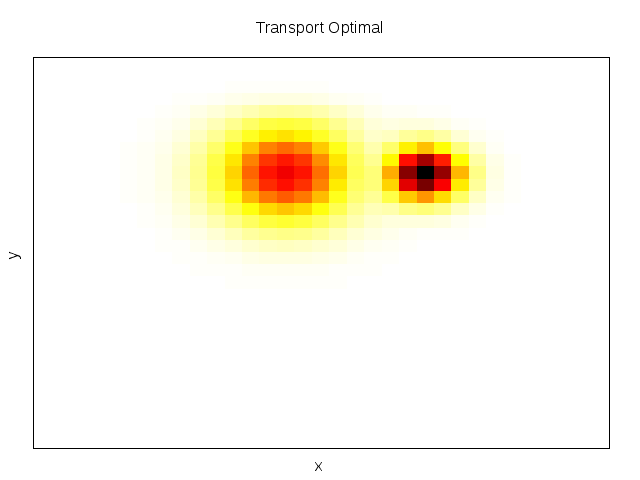
\includegraphics[width=\textwidth]{img/2DMixture/C_00028.png}
	\caption{$t=0.8$}
	\end{subfigure}
	\caption{Transport de deux gaussienne $N=P=Q=31$}
\end{figure}
\end{frame}

\begin{frame}
\vspace{-0.5cm}
\begin{figure}
\centering
\begin{tabular}{cccccc}
\rotatebox[origin=p]{90}{$\quad\qquad\ \beta = 0$} & 
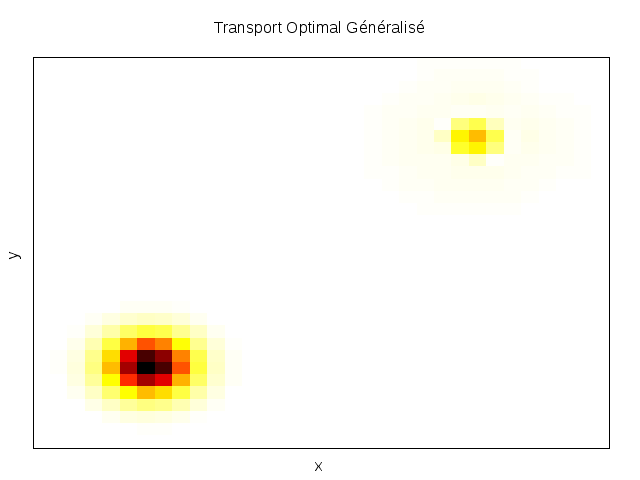
\includegraphics[width=0.15\linewidth]{img/2DGeneralise/0_C_00007.png} & 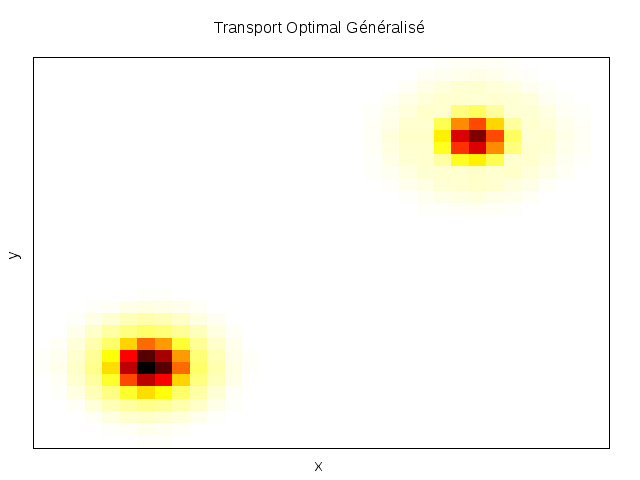
\includegraphics[width=0.15\linewidth]{img/2DGeneralise/0_C_00014.png} & 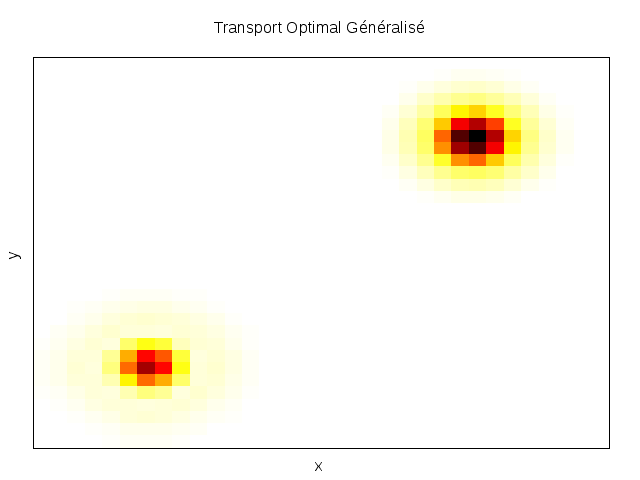
\includegraphics[width=0.15\linewidth]{img/2DGeneralise/0_C_00021.png} & 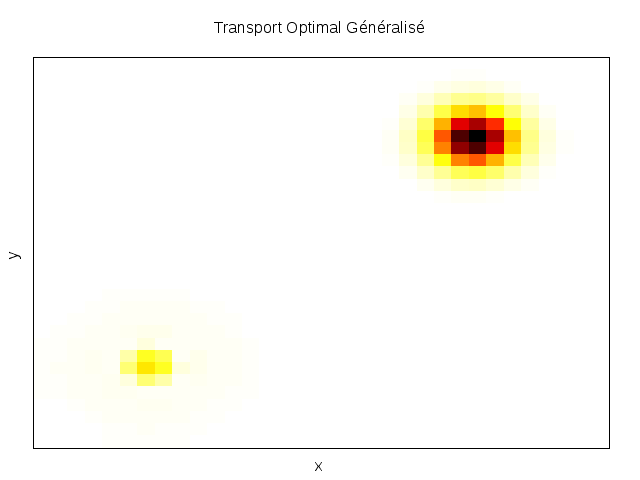
\includegraphics[width=0.15\linewidth]{img/2DGeneralise/0_C_00028.png} & \includegraphics[width=0.15\linewidth]{img/2DGeneralise/f1.png} \\ [-20pt]

\rotatebox[origin=c]{90}{$\quad\qquad\ \beta = 0.25$} &
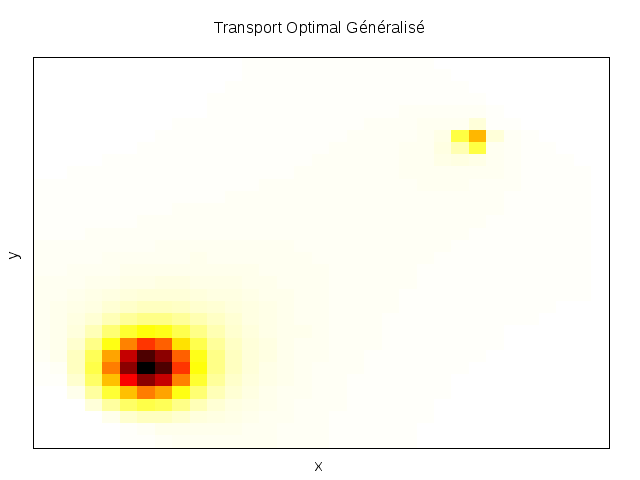
\includegraphics[width=0.15\linewidth]{img/2DGeneralise/25_C_00007.png} & 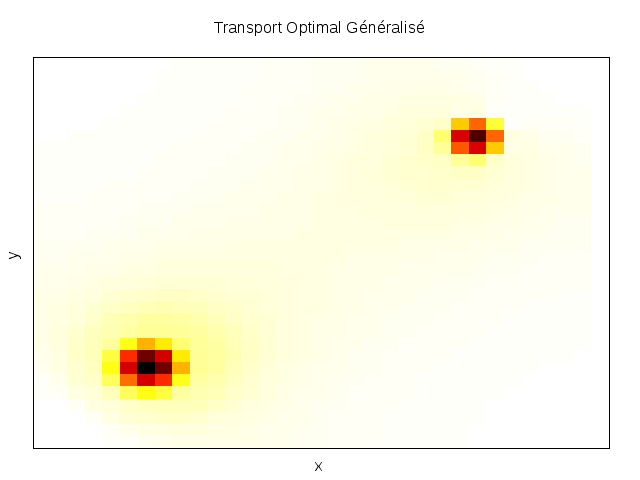
\includegraphics[width=0.15\linewidth]{img/2DGeneralise/25_C_00014.png} & 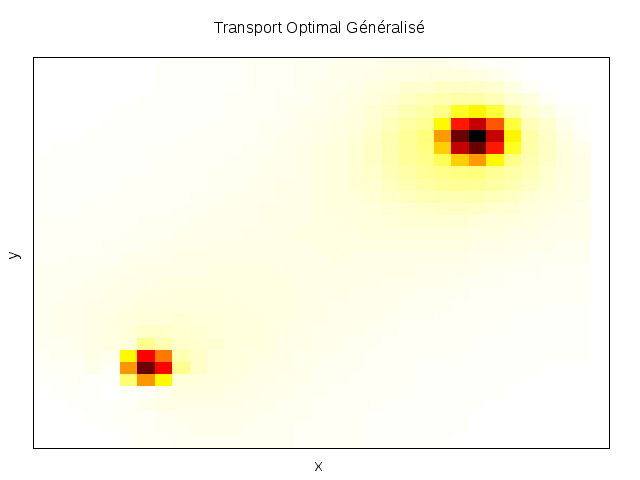
\includegraphics[width=0.15\linewidth]{img/2DGeneralise/25_C_00021.png} & 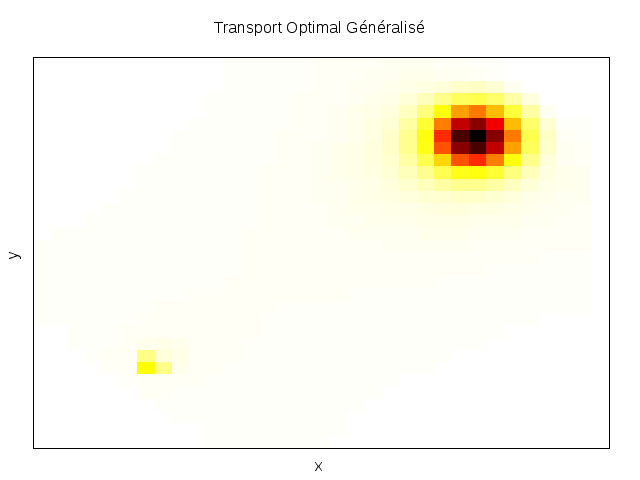
\includegraphics[width=0.15\linewidth]{img/2DGeneralise/25_C_00028.png} & \includegraphics[width=0.15\linewidth]{img/2DGeneralise/f1.png} \\ [-20pt]

\rotatebox[origin=c]{90}{$\quad\qquad\ \beta = 0.5$} &
\includegraphics[width=0.15\linewidth]{img/2DGeneralise/50_C_00007.png} & \includegraphics[width=0.15\linewidth]{img/2DGeneralise/50_C_00014.png} & \includegraphics[width=0.15\linewidth]{img/2DGeneralise/50_C_00021.png} & \includegraphics[width=0.15\linewidth]{img/2DGeneralise/50_C_00028.png} & \includegraphics[width=0.15\linewidth]{img/2DGeneralise/f1.png} \\ [-20pt]

\rotatebox[origin=c]{90}{$\quad\qquad\ \beta = 0.75$} &
\includegraphics[width=0.15\linewidth]{img/2DGeneralise/75_C_00007.png} & \includegraphics[width=0.15\linewidth]{img/2DGeneralise/75_C_00014.png} & \includegraphics[width=0.15\linewidth]{img/2DGeneralise/75_C_00021.png} & \includegraphics[width=0.15\linewidth]{img/2DGeneralise/75_C_00028.png} & \includegraphics[width=0.15\linewidth]{img/2DGeneralise/f1.png} \\ [-20pt]

\rotatebox[origin=c]{90}{$\quad\qquad\ \beta = 1$} &
\includegraphics[width=0.15\linewidth]{img/2DGeneralise/100_C_00007.png} & \includegraphics[width=0.15\linewidth]{img/2DGeneralise/100_C_00014.png} & \includegraphics[width=0.15\linewidth]{img/2DGeneralise/100_C_00021.png} & \includegraphics[width=0.15\linewidth]{img/2DGeneralise/100_C_00028.png} & \includegraphics[width=0.15\linewidth]{img/2DGeneralise/f1.png} \\ [-20pt]

& $t=0.2$ & $t=0.4$ & $t=0.6$ & $t=0.8$ & $t=1$ \\
\end{tabular}
\caption{Évolution de $f^{\star}(\cdot,t)$ pour différentes valeurs de $\beta$ et $t$. La première et la dernière image de chaque ligne sont les densités initiale et finale}
\end{figure}
\end{frame}

\begin{frame}\frametitle{Labyrinthe 2D}
Vidéo
\end{frame}
\begin{frame}\frametitle{Morphing}
Vidéo
\end{frame}


\section{Conclusion}
  
  
  
  
\end{document}
